\documentclass[12pt]{article}

%PACKAGES
\usepackage[]{graphicx}
\usepackage[english,ngerman]{babel}
\usepackage[]{color}
\usepackage{alltt}
\usepackage{mathtools}
\usepackage{dsfont}
\usepackage{amssymb}
\usepackage{amsmath}
\usepackage{MnSymbol}
\usepackage{amsmath}
\usepackage{lipsum}
\usepackage{caption}
\usepackage{subcaption}
\usepackage{amssymb}
\usepackage[a4paper, width = 160mm, top = 35mm, bottom = 30mm, 
bindingoffset = 0mm]{geometry}
\usepackage[utf8]{inputenc}
\usepackage{ragged2e}
\usepackage{xcolor}
%\usepackage[ruled,vlined]{algorithm2e}
\usepackage{fancyhdr}
\usepackage{mathrsfs}
\usepackage{algorithm}
\usepackage{algpseudocode}
\usepackage{enumitem}
\usepackage{array}
\usepackage{multirow}
\usepackage[
backend=biber,
url=false,
citestyle=nature]{biblatex}
\addbibresource{bibliography.bib}
\usepackage{hyperref}
\hypersetup{
	colorlinks = true,
	linkcolor = black,
	urlcolor = black,
	citecolor = black}

%TITLE PARAMS
\newcommand{\mytitle}{Quantification of Myogenic Differentiation Using Deep Learning}
\newcommand{\myname}{Giorgi Nozadze, Moustafa Amin, David Gorbunov}
\newcommand{\mysupervisor}{Prof. Dr. David Rügamer, Dr. Andreas Bender, Tobias Weber}
\newcommand{\mypartner}{Dr. Maximilian Saller}

\newcommand{\changefont}{%
	\fontsize{8}{11}\selectfont
}

%COMMANDS
\newcommand{\realsn}{\mathbb{R}^{\!\textit{n}}}
\newcommand{\stardist}{\texttt{StarDist}}
\newcommand{\sam}{\texttt{SAM}}
\newcommand{\with}{\qquad \text{with} \quad}
\newcommand{\integ}[2][]{\int_{#1}\mathrm{d}#2\,}
\newcommand{\reals}[1]{\mathbb{R}^{\!\textit{#1}}}
\newcommand{\identity}{\mathds{1}}
\newcommand{\expval}[2][p]{\mathbb{E}_{#1}\left[#2\right]}
\newcommand{\argmin}[2]{\underset{#1}{\mathrm{argmin}}\left(#2\right)}
\newcommand{\argmax}[2]{\underset{#1}{\mathrm{argmax}}\left(#2\right)}
\newcommand{\var}[2][p]{\text{Var}_{#1}\left[#2\right]}

\pagestyle{fancy}
\fancyhead{}
\fancyhead[R]{\changefont{\mytitle}}
\fancyfoot{}
\fancyfoot[R]{\thepage}
\setlength{\headheight}{14.5pt}
\setlength{\parindent}{0pt}
\interfootnotelinepenalty = 10000

% ------------------------------------------------------------------------------
% MAIN -------------------------------------------------------------------------
% ------------------------------------------------------------------------------
\IfFileExists{upquote.sty}{\usepackage{upquote}}{}
\numberwithin{equation}{section}
\numberwithin{figure}{section}
\begin{document}
	
	% FRONT PAGE -------------------------------------------------------------------
	
	\begin{titlepage}
		\begin{center}
			
			\LARGE
			Statistical Consulting
			
			\vspace{0.5cm}
			
			\rule{\textwidth}{1.5pt}
			\LARGE
			\textbf{\mytitle}
			\rule{\textwidth}{1.5pt}
			
			\vspace{0.5cm}
			
			\large
			Department of Statistics \\
			Ludwig-Maximilians-Universität München 
			
			\vfill
			
			\Large
			\textbf{\myname}
			
			\vfill
			
			\large
			Munich, March 1\textsuperscript{st}, 2024
			
			\vfill
			
			
\includegraphics[width = 0.4\textwidth]{sigillum.png}
			
			\vfill
			
			\normalsize
			By: \myname
						
			Correspondence email: giorginozadze23@yahoo.com
			
			Supervisors: \mysupervisor
						
			Project Partner: \mypartner

			\vfill

			
			
		\end{center}
	\end{titlepage}
 	\pagenumbering{gobble}
 	\selectlanguage{english}
\begin{abstract}
	Myogenesis, the process of muscle tissue formation and regeneration, involves the proliferation, migration, differentiation, and fusion of so called myoblasts, which ultimately form multinucleated myotubes and mature into myofibers. To gain a better understanding of myogenesis, deep learning models are proposed for accurate instance identification to quantify key metrics of individual nuclei and myotube instances in microscopy images. This approach is aimed at automating the time-consuming manual annotation process, ensuring reproducibility and eliminating human bias, while maintaining a high segmentation performance. The task consists of identifying two main objects: homogeneously shaped nuclei, for which the pre-trained \texttt{Stardist} model was used, and myotubes, which possess a very heterogeneous structure, for which a foundation model had to be employed due to the limited resources available and the lack of open source material. The Segment Anything Model (\texttt{SAM}) was developed by Meta AI and trained on over 11 million diverse images, which amounted to 1 billion masks, proved to be a promising option for this purpose, and was thus utilized in various facets of this project. Its zero-shot performance was used in a custom-built annotation tool to speed up the data labelling process and later fine-tuned to improve its recognition of myotube images, resulting in a model we call \texttt{MyoSAM}.
\end{abstract}
\selectlanguage{ngerman}
\begin{abstract}
	Die Myogenese beschreibt die Bildung und Regeneration von Muskelgewebe. Es umfasst die Proliferation, Migration, Differenzierung und Fusion sogenannter Myoblasten, die letztendlich multinukleäre Myotuben bilden und sich zu Myofasern entwickeln. Um ein besseres Verständnis der Myogenese zu erlangen, werden in dieser Arbeit Deep-Learning-Modelle vorgeschlagen, um eine genaue Instanzerkennung zur Quantifizierung wichtiger Metriken einzelner Zellkerne und Myotubeninstanzen in Mikroskopiebildern zu ermöglichen. Dieser Ansatz zielt darauf ab, den zeitaufwändigen, manuellen Annotationsprozess zu automatisieren, Reproduzierbarkeit sicherzustellen und etwaige durch Menschenhand geschaffene Verzerrungen zu eliminieren, während eine hohe Segmentierungsgüte beibehalten wird. Die Aufgabe besteht darin, zwei Arten an Objekten zu identifizieren: die homogen geformten Zellkerne, für die das vortrainierte \texttt{Stardist}-Modell verwendet wurde, und die Myotuben, die eine sehr heterogene Struktur aufweisen, für die aufgrund der begrenzten Ressourcen und des Mangels an Open-Source-Daten ein Foundationmodell eingesetzt werden musste. Das von Meta AI entwickelte und auf über 11 Millionen verschiedenen Bildern und entsprechend über einer Milliarde Masken trainierte Segment-Anything-Modell (\texttt{SAM}) hat sich als vielversprechende Option für diesen Zweck erwiesen und wurde daher auf verschiedene Weise genutzt. Seine Zero-Shot-Performance wurde in einem benutzerdefinierten Annotationswerkzeug verwendet, um den Prozess der Datenbeschriftung zu beschleunigen, und später feinjustiert, um die Erkennung von Myotubenbilder zu verbessern, was zu einem Modell, das wir MyoSAM nennen, führte.
\end{abstract}
\selectlanguage{english}
 	\listoffigures
 	\listoftables
 	\clearpage
	\tableofcontents
	\newpage
	\pagenumbering{arabic}
	\setcounter{page}{1}
	\newpage
	\section{Background and Project Goal}
Myogenesis is the process that describes the formation, growth, development as well as regeneration of muscle tissues in the body. In detail, mononucleated, partially differentiated precursor cells, also called myoblasts, proliferate, migrate, differentiate, align, fuse to ultimately form multinucleated myotubes. In their quiescent state, myoblasts are called myosatellite cells and require mechanical stress for activation. In vivo, myotubes mature into myofibers that stretch along the entirety of skeletal muscles \cite{tajbakhsh2009, bentzinger, bollen}.

Several diseases such as sarcopenia, muscle dystrophy, obesity, or diabetes severely affect the physiological homeostasis and lead to a loss of skeletal muscle mass and function (muscle atrophy) \cite{argiles}. In contrast, physical activity does not just lead to an increase of muscle mass and function (muscle hypertrophy), but also reduces glucose levels and lipid accumulation. Treatment of diseases that lead to muscle atrophy often requires a multifactorial approach. Therefore, candidate compounds, genes, proteins or metabolites are initially analyzed in large-scale in vitro experiments utilizing myoblast cell lines such as murine C2C12 cells \cite{bajaj}.

Given the spatiotemporal nature of myogenesis, it is crucial to identify and quantify individual myoblasts and fused myotubes in microscopy images to evaluate the effect of each compound or biological molecule on myoblast fusion or atrophy/hypertrophy. Other than simply counting the number of each cell type, the creation and morphological quantification of individual myotube masks enables a thorough analysis of several other biologically relevant parameters such as the differentiation state/extend or myotube area and diameter in addition to interaction of different myoblasts. Unfortunately, the manual creation of individual cell masks in large-scale experiments is tremendously time consuming and might take months to finish. Therefore, this project intends to obtain such quantitative statistics without resorting to heuristics by using two different instance segmentation models for cell nuclei and myotubes.

These models need to overcome two hurdles. First and foremost, it must be able to differentiate between overlapping instances. Besides coincidence, these overlaps might be caused by myogenesis itself or due to the threedimensional nature of the cells caused by acutal overlapping myotubes. Secondly, it should be robust in its predictions. Many times, microscopy images require preprocessing that can create artifacts by amplifying noise or blurring small scale structures. Therefore, the instance segmentation should aim to be as independent of the preprocessing as possible.

Taken together, the goal is not only to speed up otherwise time-consuming analyses, but also to improve reproducibility and eliminate all human bias within the process of instance segmentation. Human bias can occur at various points. Many times, it is difficult to distinguish whether a continuously bright region is one object or several ones. Furthermore, the quality of preprocessing can influence the number of counted cells because some instances may be too dim too spot with the naked eye.

	\newpage
	\section{Segmentation using Unsupervised Methods}\label{secunsupervised}
In the beginning, established, unsupervised methods were used to segment the images in order to gain a better understanding of the data. Unsupervised learning includes algorithms which intend to find regularities, structures, or patterns within unlabeled datasets. As they require no ground truth labeled data and are not too computationally expensive, they are a great fit for exploratory analysis. The results of two classical methods (watershed and ellipse fitting) applied to the given images are discussed in the following. For this section, one myotube-myoblast image pair in Fig.~\ref{figtubeblast} and Fig.~\ref{figoverlap} will be used to exemplify the unsupervised methods. The following figures within this section where created using \texttt{OpenCV} \cite{opencv_library}.
\begin{figure}
	\centering
	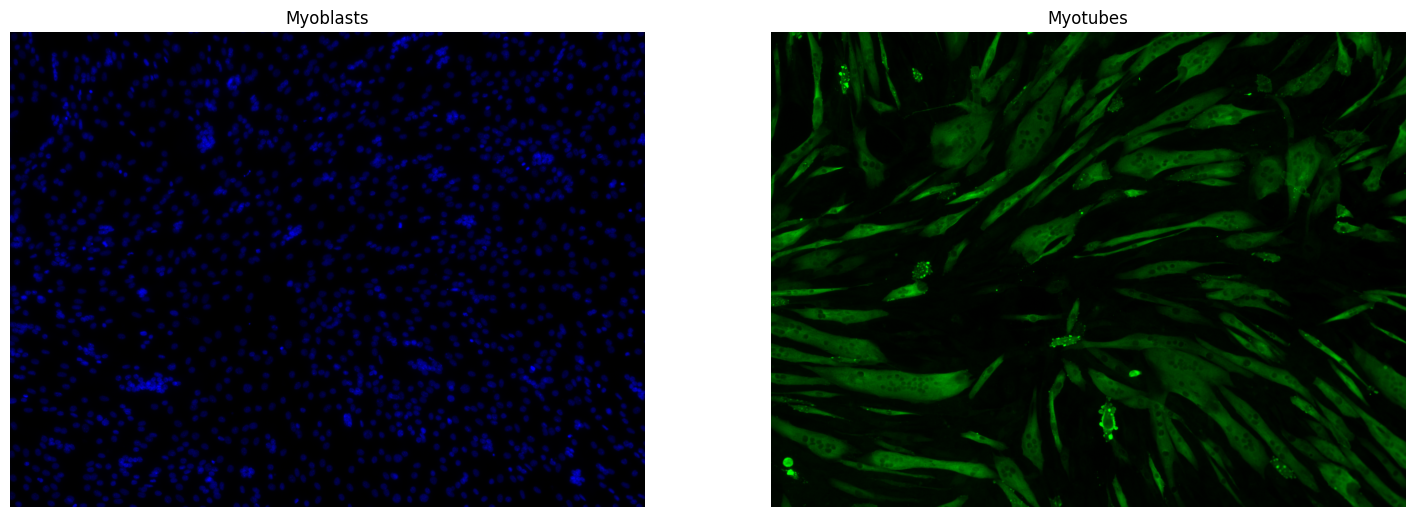
\includegraphics[width=\textwidth]{"images/workhorse.png"}
	\caption[Workhorse image of myoblasts/cell nuclei and myotubes]{Microscopy image of myotubes and myoblasts/nuclei. In this juxtaposition it is clearly visible that some myoblasts form the nuclei of the myotubes due to the dark circles within them.}
	\label{figtubeblast}
\end{figure}

\begin{figure}
	\centering
	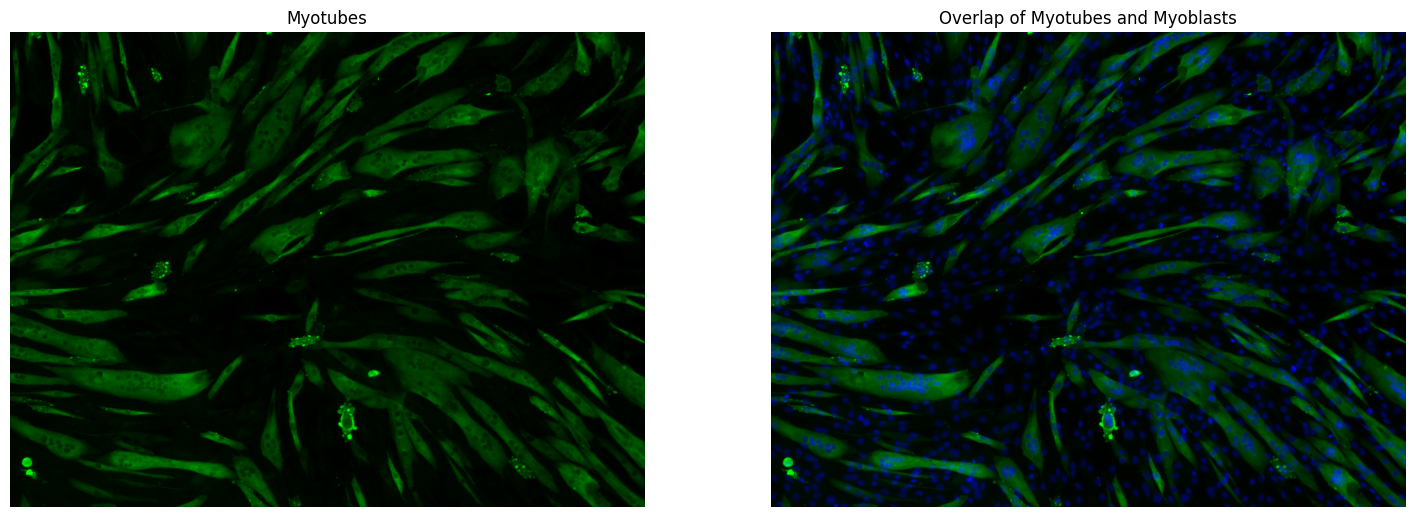
\includegraphics[width=\textwidth]{"images/overlap.png"}
	\caption[Overlap of myoblasts/cell nuclei and myotubes]{Overlap of myoblasts and cell nuclei and myotubes. It clearly shows which nuclei have fused into myotubes.}
	\label{figoverlap}
\end{figure}

\subsection{k-Means Clustering and Otsu Thresholding}
As a starter, foreground detection algorithms were tried out in order to discriminate between cells, be it myotubes or myoblasts, and background. There are two common methods to do so in computer vision. 

The first one is the k-Means algorithm, whose goal it is to minimize the within-class-variance of a (predetermined) number of $k$ clusters \cite{bishop2006}. To this end, $k$ points are initialized and function as the first centers of the clusters. All observations are then grouped by proximity to the centers (according to some distance measure, commonly the $L2-$norm). This procedure is reiterated until convergence. In its simplest form, all initial points are drawn from a uniform distribution. A more common implementation is the k-Means++ algorithm \cite{kmeans} which samples only one point from a uniform distribution. All other points are sampled from a distribution proportional to the (squared) distance to the first point so as to minimize the chance of drawing cluster centers close to one another.

In order to use k-Means for image segmentation, the image first needs to be transformed to grayscale. Upon calculating the histogram of pixel intensities, the counts for every bin take the roles of the observations. Using $k = 2$ results in one threshold value seperating two intervals. All pixels with values above this threshold are considered foreground, all the other ones are background.

In a similar vein, Otsu's method \cite{otsu} was utilized. In many ways, Otsu thresholding is not too different from k-Means in the sense that it also minimizes within-class-variance of the grayscale histogram. They can even be shown to be equivalent but only the Otsu method guarantees convergence to the global optimum \cite{liu2009otsu}. Implementation wise, variance estimates are calculated explicitly by iterating the threshold over all possible grayscale values to find the optimal one with respect to the within-class variance as the objective function.

Both foreground detection algorithms applied to Fig.~\ref{figtubeblast} can be found in Fig.~\ref{figkmblast}-\ref{figotsutube}. While this is not instance segmentation per se and therefore one cannot distinguish between overlapping cell instances, it is very helpful to gain intuition on the available images by evaluating the resulting connected components. One major drawback of thresholding methods is the fact that a hard cutoff implies that instances that are too dim are taken to be background.
\begin{figure}
	\centering
	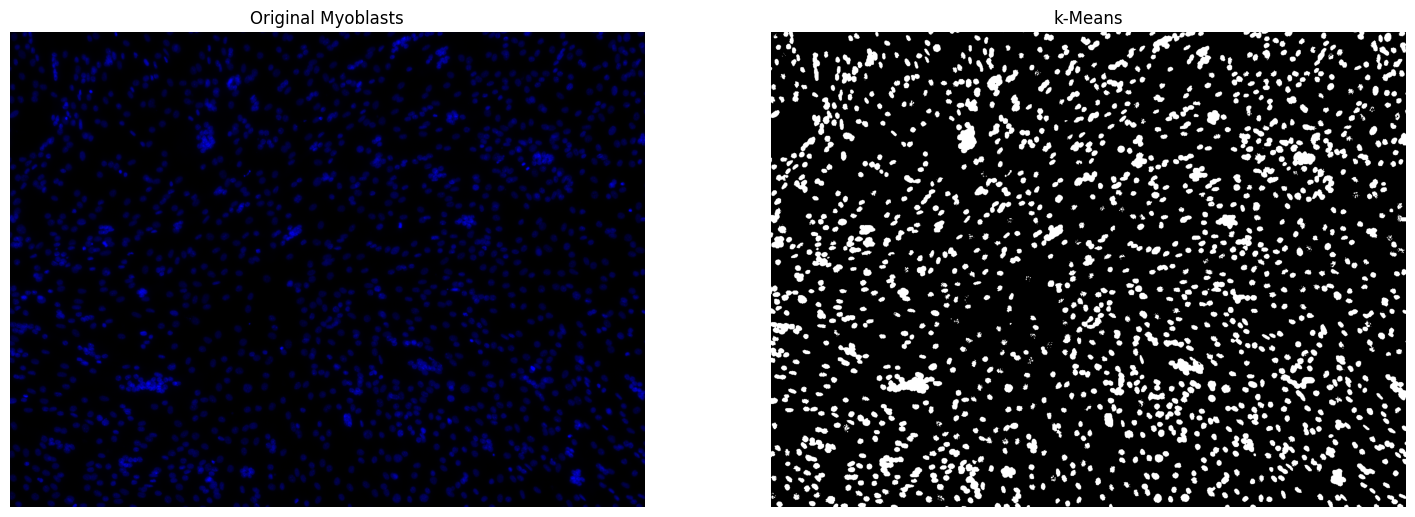
\includegraphics[width=\textwidth]{"images/km_blast.png"}
	\caption[k-Means applied to nuclei]{Foreground detection of myoblasts and cell nuclei using k-Means}
	\label{figkmblast}
\end{figure}
\begin{figure}
	\centering
	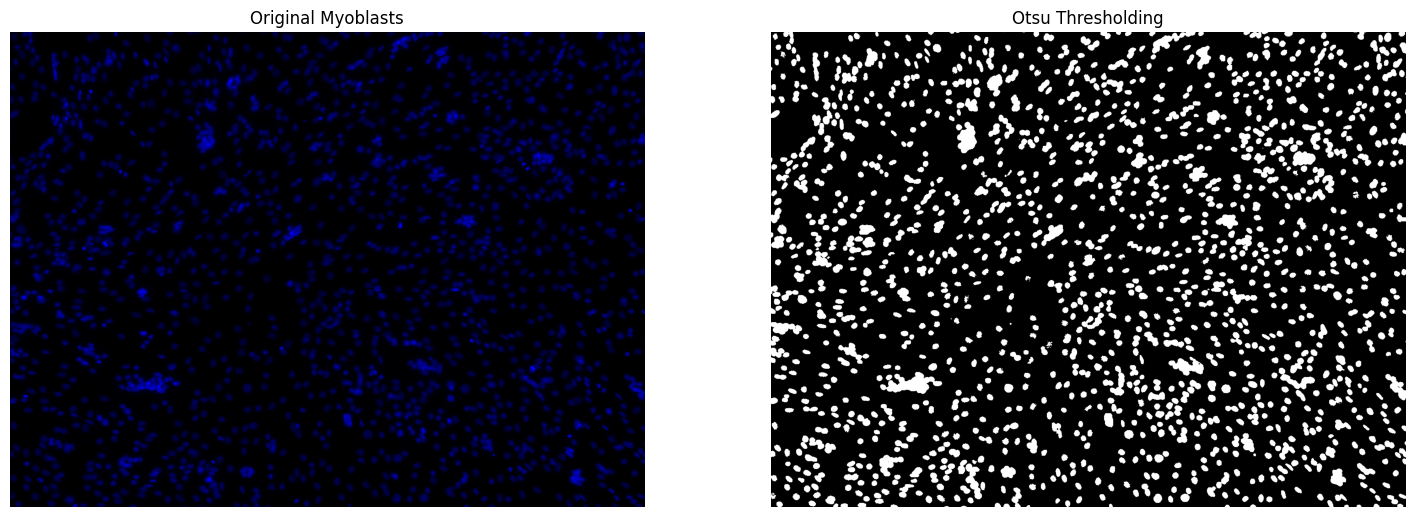
\includegraphics[width=\textwidth]{"images/otsu_blast.png"}
	\caption[Otsu thresholding applied to nuclei]{Foreground detection of myoblasts and cell nuclei using Otsu thresholding}
	\label{figotsublast}
\end{figure}
\begin{figure}
	\centering
	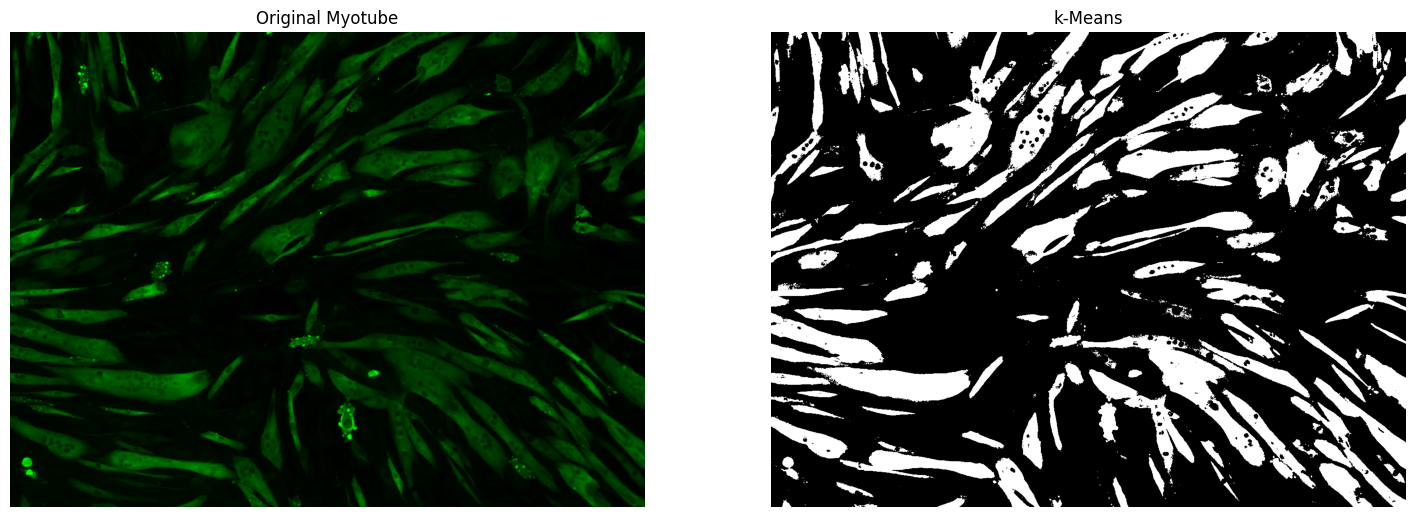
\includegraphics[width=\textwidth]{"images/km_tube.png"}
	\caption[k-Means applied to myotubes]{Foreground detection of myotubes using k-Means}
	\label{figkmtube}
\end{figure}
\begin{figure}
	\centering
	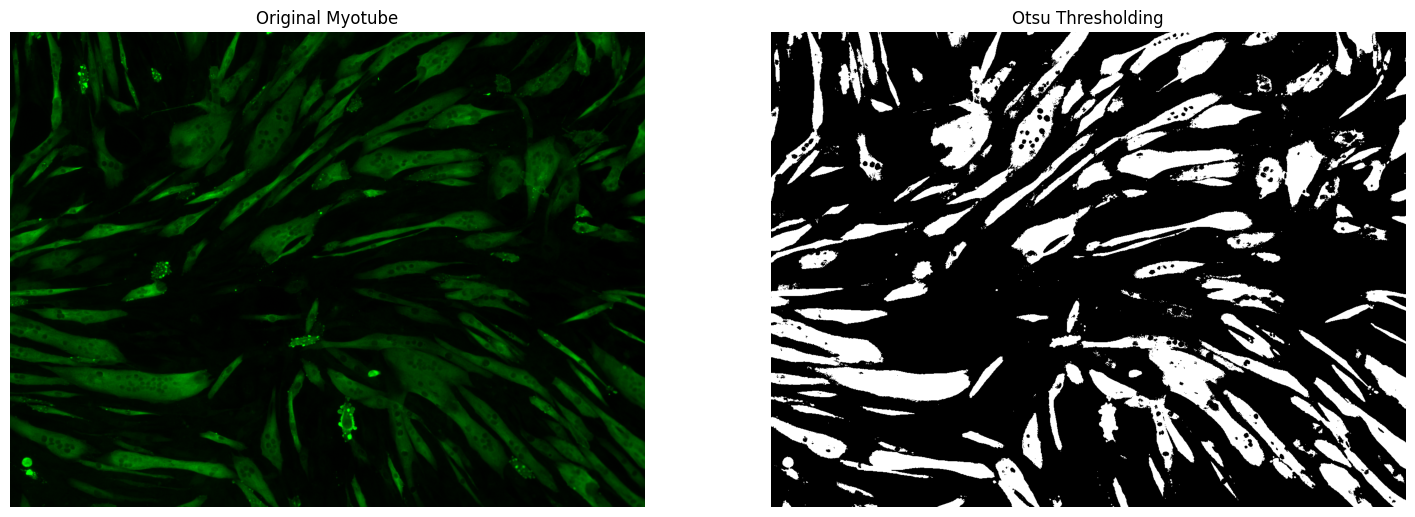
\includegraphics[width=\textwidth]{"images/otsu_tube.png"}
	\caption[Otsu thresholding applied to myotubes]{Foreground detection of myotubes using Otsu thresholding}
	\label{figotsutube}
\end{figure}
\newpage
\subsection{Edge Detection}
As a further attempt to obtain instances of the cells, Canny edge detection \cite{canny} was employed in the hopes that overlapping instances have clear enough borders to be individually identified. In the Canny edge detection algorithm, a Gaussian filter is applied to the image to smooth out any noise present in the image. Next, the intensity gradients of the image are computed highlighting regions of significant change in intensity. The gradient thereby serves as a proxy for the edges. In this case, the Sobel filter \cite{Gonzalez1992} was used to estimate the image gradient. To further refine the edge detection, lower bound cut-off suppression is employed to thin out edges and retain only strong, relevant ones. This is accomplished by iterating over all non-zero pixels in the gradient image and checking whether it is a local minimum among its eight neighbors. Following this, a double thresholding technique is utilized to classify pixels as potential edge pixels or non-edge pixels based on their gradient magnitudes. The lower value defines a hard cut-off such that every gradient pixel below that value is set to zero. Any pixel value greater than the larger value defines a strong edge. If a pixel is between the chosen values, the pixel is assumed to be part of a weak edge. Weak edges are only kept if they are connected to strong ones. This is also known as hysteresis thresholding. This multi-step process ensures robust edge detection, particularly in scenarios where noise levels vary or edges are fragmented.
\begin{figure}
	\centering
	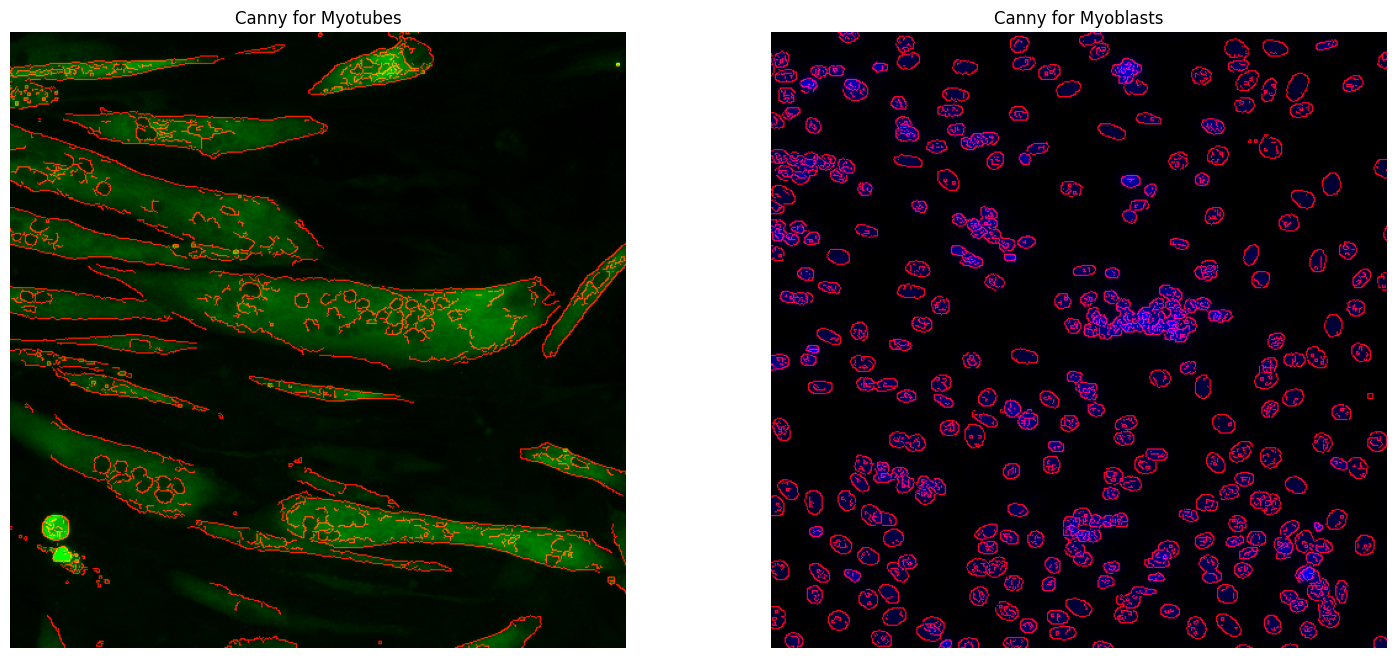
\includegraphics[width=\textwidth]{"images/canny.png"}
	\caption{Canny edge detection applied to both microscopy images.}
	\label{figcanny}
\end{figure}

But yet again, this approach is not particularly desirable because obtaining decent segmentations from it requires a lot of tuning of hyperparameters as well as preprocessing and postprocessing steps tailored to every indivdual image (in addition to running the Canny algorithm in and of itself). Furthermore, the Canny algorithm by itself has many tunable parameters and also possesses the downsides that come with thresholding.
\newpage
\subsection{Watershed}
Little math is necessary to understand how segmentation using watersheds functions. First, the image needs to be transformed to grayscale because the resulting single channel needs to be thought of as the a third dimension defining a height profile or topography. In case of a uint8 encoding, the height may take values between 0 and 255. Each pixel can be either of the three following types: a (regional) minimum, a catchment basin or watershed of that minimum, or watershed lines. The first type of pixel is self-explanatory. Continuing with the metaphor, a pixel of the second or third type can be thought of in the following manner: picture the position and intensity of the pixel as defining the starting point on the 3d topography defined by the grayscale image. Placing a drop of water on this location can either have it run down (second type) or stay put (third type). All the points where water would run downhill are known as watersheds. All the other points that are not minima define crests, which are the divide (or watershed) lines, beyond which water would not move at all. Iterating over possible intensities starting from the lowest one in the image, or, by analogy, flooding the 3d landscape by poking a hole in the minimum, defines connected areas, or collections of water within a basin, around every regional minimum. Continued flooding will have the water level rise until the first two connected areas merge into one. To prevent that, a dam, whose locations define the pixels of the watershed lines, would need to be built. How to properly construct such dams by means of morphological operations \cite{serra} is thoroughly explained in \cite{Gonzalez1992, coupriewatershed}. The resulting watershed lines are then interpreted as the boundaries of an instance. In this case, a marker-based approach to watershed \cite{meyer} was opted for. Therein, before applying the watershed algorithm, the identification of markers, which are typically connected patches of pixels that represent objects of interest, is necessary. These markers determine where the flooding begins. 

Based on this intuition, two observations can be made. Firstly, on first glance a catchment basin can have the shape of a myotube or cell nuclei making watershed a sensible segmentation method. Secondly, this method requires the instances to have low grayscale values. This implies that images need to be processed before applying the watershed algorithm since cells are accumulations of high intensity areas. The most naive approach would be a simple inversion of the image. But this can lead to oversegmentation due to noisy sections. More sophisticated approaches either are based on image gradients or a distance transform applied to a binary representation of the original image. The former approach is used in this report and its result will be shown before long.

Just from these theoretical discussions alone, it becomes evident that the algorithm will have a hard time differentiating between merging nuclei because they presumably will be interpreted as one single catchment basin due to their intesities being similar. Therefore it still is very difficult to resolve sizable overlaps, unless of course the markers are set such that the algorithm knows that they are different a priori. So again, the results will heavily rely on the quality of preprocessing which presents a unique challenge for every new image and something that is ideally avoided. All of these problems are glaringly obvious when applied to the typical images in Fig.~\ref{figwatershed}.

\begin{figure}
	\centering
	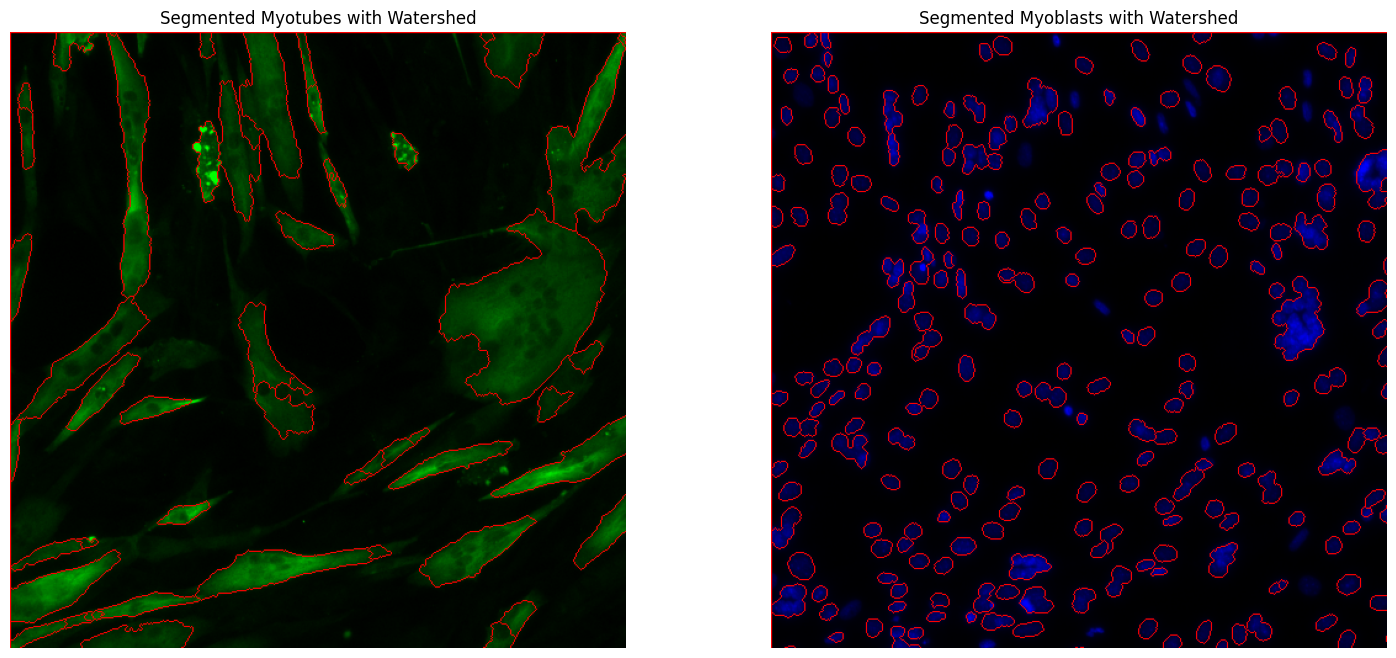
\includegraphics[width=\textwidth]{"images/watershed.png"}
	\caption[Application of watershed]{Marker-based watershed applied to both microscopy images.}
	\label{figwatershed}
\end{figure}

\newpage
\subsection{Ellipse Fitting}
As a last resort for unsupervised methods, it was attempted to fit ellipses to the nuclei/myoblast images. It is evident that this approach would not work for myotubes due to their oftentimes crooked shapes. But for a typical myoblast image, it does seem to be a sensible approximation. There are several methods that are based on a similar intuition in the literature \cite{panagiotakis2020region, panagiotakis2018cell, kothari2009automated}. All of them have a common structure. The image is preprocessed, which usually consists of methods previously delineated in this section like thresholding, Gaussian filtering, edge detection but also other things like hole-filling. Therefore it can be assumed that the typical foreground detection has been performed. At this point, methods start diverging. In some cases ellipses are fit based on the curvature of the foreground. In other cases, many ellipses are fit and the fit with the highest goodness measure like AIC is kept. In addition to that, there are some computed quantities determining whether a segment is large, small, circular, or bright enough to be a cell. All in all, the final part distinguishes touching and overlapping cells one way or another. But even with all these things considered, the segmentation quality is easily influenced by the chosen preprocessing, as can be seen in Fig.~\ref{figellipsefitting}. 
\begin{figure}
	\centering
	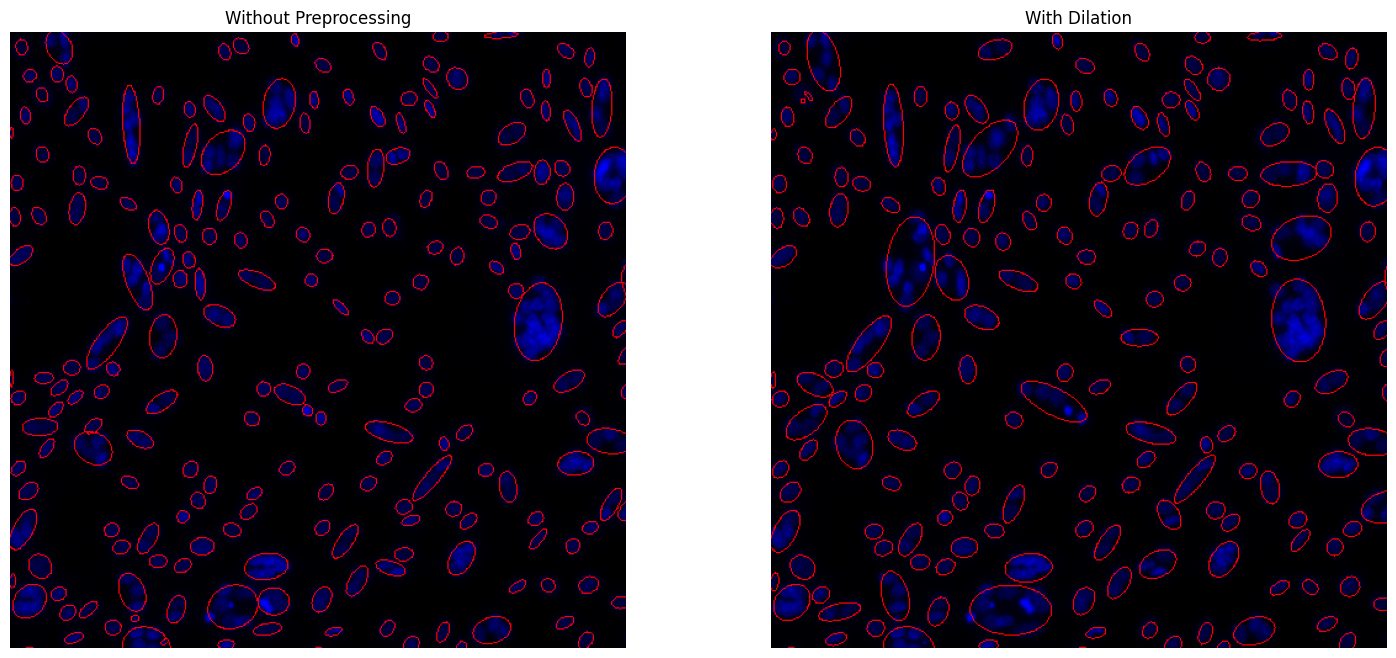
\includegraphics[width=\textwidth]{"images/ellipsefitting.png"}
	\caption[Ellipse Fitting as segmentation]{Ellipse fitting for nuclei/myoblasts. One additional application of a dilation operation markedly alters the outcome of the segmentation.}
	\label{figellipsefitting}
\end{figure}

	\newpage
	\section{Myoblast Segmentation using \stardist}\label{secstardist}
As discussed in Sec.~\ref{secunsupervised}, typical instance segmentation methods suffer from the suppresion of valid objects or the merging of instances given overlaps. In order to better segment the myoblasts, a cell detection method called \stardist \cite{schmidt2018, weigert2020} is used. It was developed with the intent to segment microscopy data like the nuclei found in this project. A deep learning model would have the advantage of being flexible enough to not require much preprocessing and can ideally be used out-of-box if there exists a pretrained model.
\subsection{\texttt{StarDist} Background}
In brief, a convolutional neural network is trained to predict polygons imitating typical cell shapes for every pixel of the image. More concretely, it predicts a star-convex polygon for every (non-background) pixel. Intuitively speaking, a star-convex set $\mathcal{S}$ is one where there exists one point $s_{0}$ such that for every point $s \in \mathcal{S}$ the line segment connecting $s_{0}$ to $s$ is element of $\mathcal{S}$. Such a shape can be approximated by following $n$ predefined radial directions for a distance of $\{r^{k}\}^{n}_{k = 1}$ starting from a point $s_{0}$. This better approximates the myoblast shape than ellipses. The training data contains pairs of both raw and fully annoted label images in the sense that every pixel either has a unique object identifier or is marked as background. Given the annoted images, it is possible to compute the radial distances $\{r^{k}_{ij}\}^{n}_{k = 1}$ to the assigned object's boundaries starting at every single foreground pixel parametrized by $i, j$ serving as the point  $s_{0}$. Furthermore, for every single foreground pixel the Euclidean distance to the closest background pixel is computed. Normalizing this distance gives a value $d_{ij}$ between 0 and 1 interpreted as a probability to be a foreground point. The calculations are visualized in Fig.~\ref{figstardistexplained}. At the end of the day, both object probabilities and the $n$ distances are predicted for each image and denoted with $\hat{d}$ and $\hat{r}$ respectively. The object probabilities are penalized according to the binary cross entropy loss

\begin{equation}\label{eqbceloss}
	L_{\text{obj}}(d,\hat{d})=-d\log\hat{d}-(1-d)\log(1-\hat{d}),
\end{equation}
and the object probability weighted mean absolute error is used as a loss
\begin{equation}
	L_{\text{dist}}(d,\hat{d},r_k,\hat{r}_k)=d\cdot\frac{1}{n}\sum_k|r_k-\hat{r}_k|,
\end{equation}
for the radial distances. This implies that the further a point is away from an object boundary, the more it contributes to the loss and background pixels do not contribute at all.
\begin{figure}
	\centering
	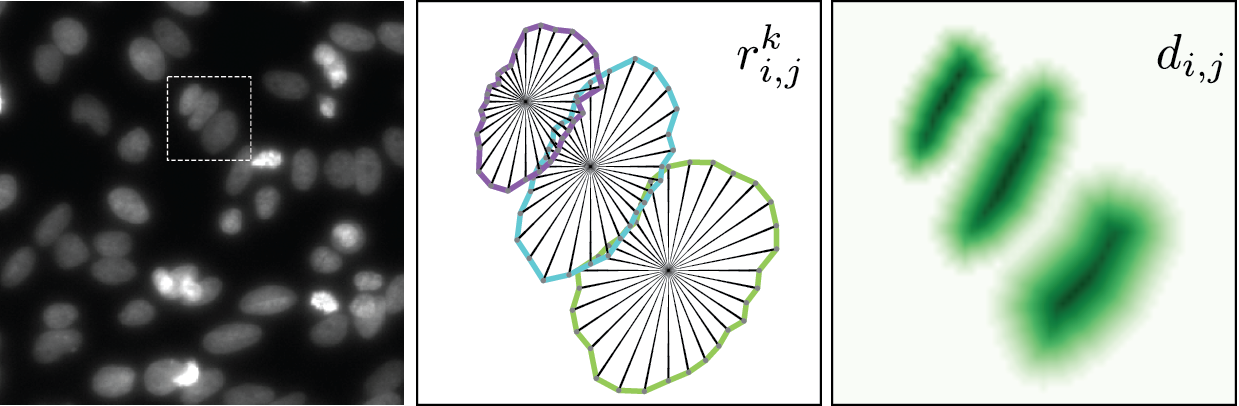
\includegraphics[width=\textwidth]{"images/star_convexity_explained.png"}
	\caption[\texttt{StarDist} summarized]{Example of an area that is complicated to segment due to overlaps. \texttt{StarDist} creates the segementation by forming star-convex polygons and computing the probability to belong to said instance. Source: \Cite{schmidt2018}.}
	\label{figstardistexplained}
\end{figure}

In \stardist, the \texttt{U-Net} architecture \cite{RonnebergerFB15} is used as the backbone and is slightly modified by adding another 128-channel 3x3-convolutional layer with ReLu activation to the \texttt{U-Net} output in order to add a lot of flexibility to the network. This output, in turn, is fed into two other convolutional layers. The first one it is input into is a single channel convolutional layer with sigmoid activation meant to learn object probabilities. The second one has a linear activation and as many channels as there are radial directions. In total, $n+1$ values are predicted for each pixel. Presumably, two points close by will learn two similar representations for the same instance, a way too remove redundant predictions is needed. This is accomplished through non-maximum suppression (NMS) \cite{hosang2017learning, ren2016faster} where only polygons associated with high probability pixels are taken into account.
	\newpage
	\section{Segmentation of Myotubes with \texttt{MyoSAM}}\label{secsam}

Myotube and cell nuclei microscopy images significantly differ from natural images. While cell nuclei images tend to be more homogeneous in size and shape of the nuclei, presenting recurring problems, myotube images exhibit far greater diversity. Our exploratory data analysis aimed to understand the characteristics of myotube images, both quantitatively and qualitatively.

\paragraph{Qualitative Analysis}
\begin{figure}
	\centering
	\includegraphics[width=\textwidth]{"images/myotube_image_set.png"}
	\caption[Sample myotube images]{Sample of myotube images of varying sizes.}
	\label{figsamplemyotubes}
\end{figure}
\ \\
In the myotube image set eventually used for training, it is clear that the images vary widely in size, brightness, and color schemes. They are primarily monochromatic, with their color depending on the biomarker used and the type of microscope employed for capturing the images (cf. Fig.~\ref{figsamplemyotubes}). Additionally, the myotubes themselves display considerable variation in size, shape, and density. This variety underscores the diverse data distribution present within myotube images as a whole.

\paragraph{Quantitative Analysis}
\ \\
Upon evaluating the images selected for training, we found that myotube images are predominantly dark. The evaluated images had average red, green, and blue values of 2.56, 9.8, and 2.9, respectively, with a high degree of variance. Further analysis into the HSL (Hue, Saturation, Lightness) space of these images confirmed their darkness, primarily attributed to the large areas of dark background present. Fig.~\ref{figrgb}, Fig.~\ref{fighsl} and the table below summarize the activations for red, green, blue, and lightness across several images.

\begin{tabular}{|p{2cm}|p{2cm}|p{2cm}|p{2cm}|p{2cm}|p{2cm}|}
	\hline
	& Minimum Activation & Minimum non-zero  activation & Maximum activation & Mean of mean activations & Mean of activation standard deviations \\
	\hline
	Red & 0 & 1.89 & 6.90 & 2.56 & 3.88 \\
	\hline
	Green & 0 & 1.89 & 28.34 & 9.79 & 8.13 \\
	\hline
	Blue & 0 & 2.84 & 17.48 & 2.90 & 2.36 \\
	\hline
	Lightness & 0.64 & NA & 14.23 & 5.37 & 4.75 \\
	\hline
\end{tabular}

\begin{figure}
	\centering
	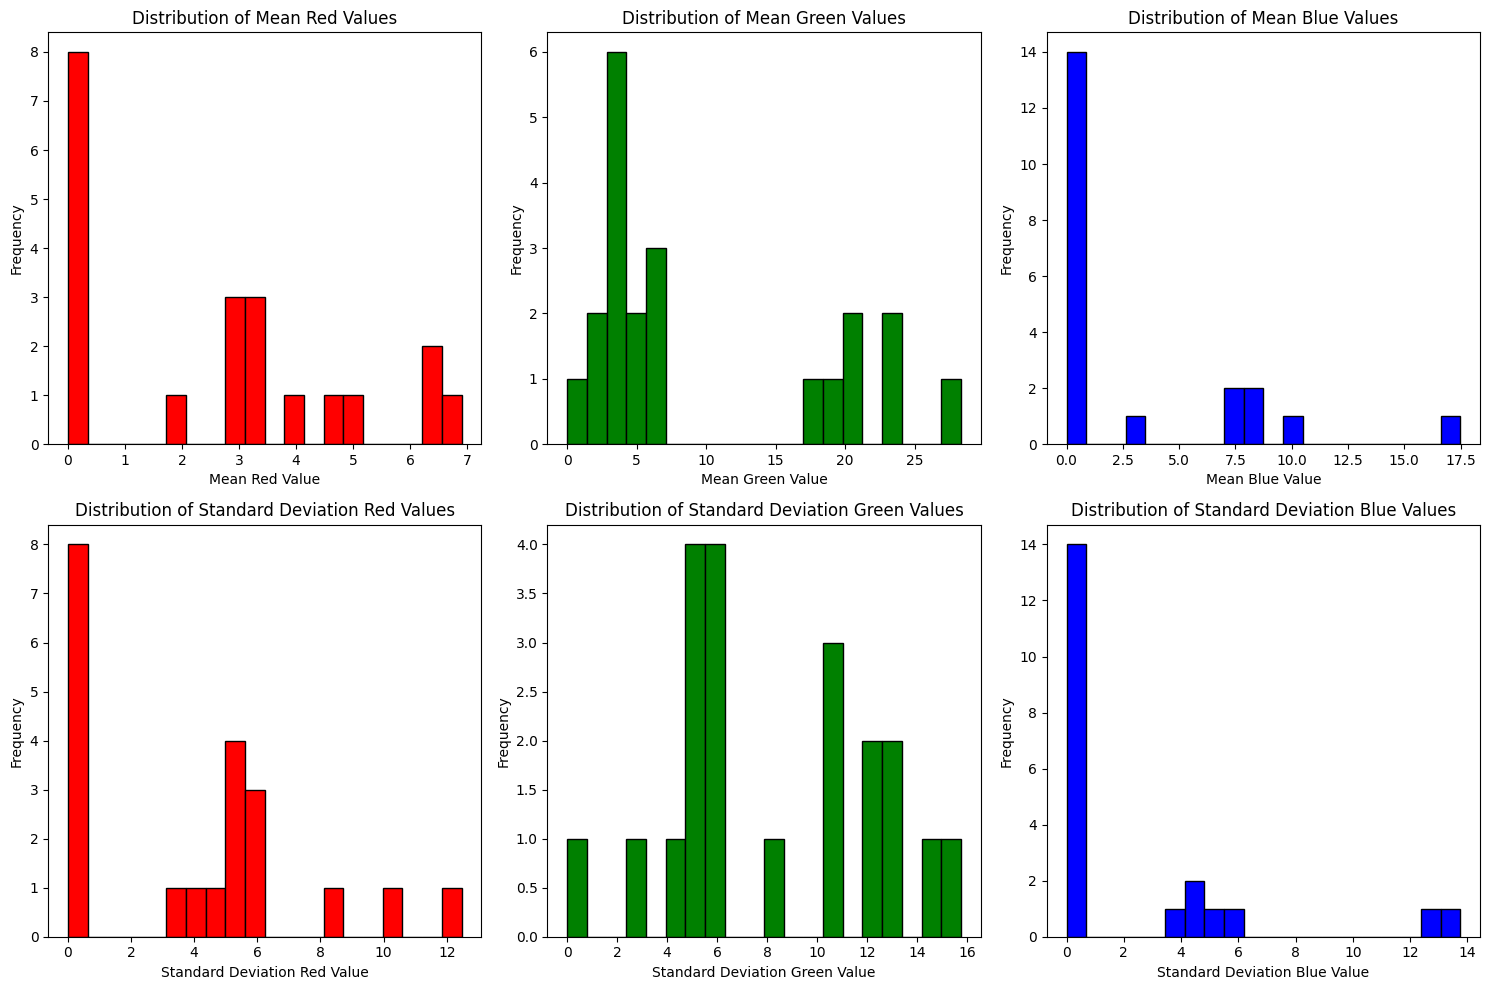
\includegraphics[width=\textwidth]{"images/pixel_distribution_plots_rgb.png"}
	\caption[Myotube RGB activation distribution]{Activation of RGB channels in the myotube training dataset.}
	\label{figrgb}
\end{figure}
\begin{figure}
	\centering
	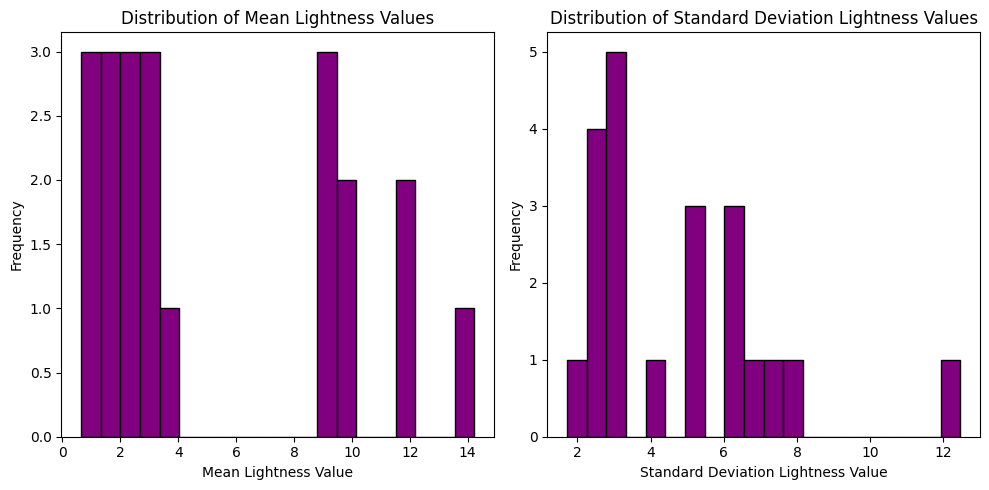
\includegraphics[width=\textwidth]{"images/pixel_distribution_plots_hsl.png"}
	\caption[Myotube lightness activation distribution]{Activation of lightness channel from HSL space in the myotube training dataset.}
	\label{fighsl}
\end{figure}
\ \\
This analysis highlights the necessity of treating myotube images differently from natural images. For instance, typical normalization techniques based on pixel activation means derived from natural images are not directly applicable to myotube images due to their unique characteristics.

Alas, typical myotubes cannot be represented as star-convex polygons since oftentimes they have slight constrictions (cf. Fig.~\ref{figtubeblast}) or even bifurcations.

Recently, the Segment Anything Model (SAM) \cite{kirillov2023segment} developed by Meta AI has demonstrated great promise in the field of natural image segmentation. Trained on the largest segmentation dataset to date, encompassing over 11 million diverse images and 1 billion corresponding masks, this model benefits from both the scale and quality of the dataset. With its powerful transformer-based architecture, \texttt{SAM} has gained a comprehensive understanding of objects, enabling it to achieve exceptional zero-shot performances, sometimes even surpassing fully supervised models.
Despite the significant progress made within the zero-shot framework, challenges arise when applying \texttt{SAM} to more specialised domains such as medical and satellite imaging. Due to the underrepresentation of images from these domains in the training data, the model is not as precise as desired. For instance, as illustrated in Fig.~\ref{figzeroshot}, \texttt{SAM} struggles with identifying overlapping myotubes. Moreover, in scenarios where segmentation of only specific critical areas is required, using \texttt{SAM} can be overwhelming as it attempts to “segment anything” it detects, including background, small artifacts, small nuclei cells within myotubes, and edges of the image. To address these challenges and enable a fully automatic instance segmentation process, fine-tuning the model was necessary, leading to a model we dubbed Myovision Segment Anything Model (\texttt{MyoSAM}).

\begin{figure}
	\centering
	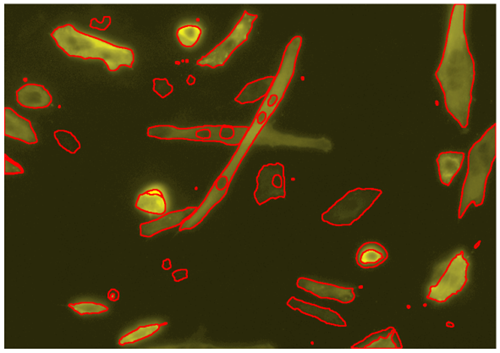
\includegraphics[width=\textwidth]{"images/sam_zeroshot.png"}
	\caption[\texttt{SAM} zeroshot]{Out-of-box application of the pretrained version of \texttt{SAM} to one patch of a myotube image.}
	\label{figzeroshot}
\end{figure}
\subsection{\texttt{SAM} Background}\label{SAMbg}
The strong generalization capability of the \texttt{SAM} was achieved through careful design of its task objective, model architecture, and dataset used in training. The goal of the Meta AI research team was to develop a model capable of generalizing across various downstream computer vision tasks and data distributions, including instance segmentation, edge detection, and object suggestions, among others.

Meta AI's reserchers drew inspiration from how humans would perform the aforementioned tasks. Drawing parallels to the human ability to adapt to various tasks through acquired expertise within a specific domain, one would typically present a person with an image alongside some form of guidance on what is expected. This guidance could be a direct indication of the object to segment, such as pointing to it, creating boundaries around it with a box or a mask, or providing instructions in text form, especially when face-to-face communication isn't an option.

Initially, the human would discern and isolate the object, subsequently carrying out the tasks as directed. These guiding signals are termed “prompts“, a concept adapted from the field of Natural Language Processing (NLP). The Meta AI Research Team has termed this versatile task \textit{promptable segmentation task}. It involves providing an image and a prompt to produce a segmentation mask for the specified object, which then can be utilised for a variety of downstream tasks. However, there is an added layer of complexity: the model should be capable of formulating multiple segmentation masks from a single prompt. This is because prompts may be vague and potentially applicable to multiple objects within an image. For instance, a prompt might relate to a person, a bag, or even a zipper on the bag. Despite the ambiguity, the model is expected to generate at least one meaningful mask corresponding to one of the objects the prompt refers to.
Such a promptable segmentation task inevitably imposes specific constraints on the possible model architectures. The model must be capable of processing an image as input while simultaneously encoding various forms of prompts. It must then combine these two streams of information to accurately predict the segmentation mask. Additionally, the integration of image and prompt inputs must be designed efficiently in a fashion so as to allow real-time interactive segmentation. 
Meta AI devised a distinctly clear model architecture that satisfies all the outlined constraints effectively. The model consists of image encoder, prompt encoder, and a lightweight mask decoder. A high-level overview of \texttt{SAM} can be gained through Fig.~\ref{figsamoverview}.

The broad idea behind the model is simple: there needs to be a way to independently embed both prompt and image in order to jointly predict masks. The model therefore mainly consists of image encoder, prompt encoder, and a decoder network.
\begin{figure}
	\centering
	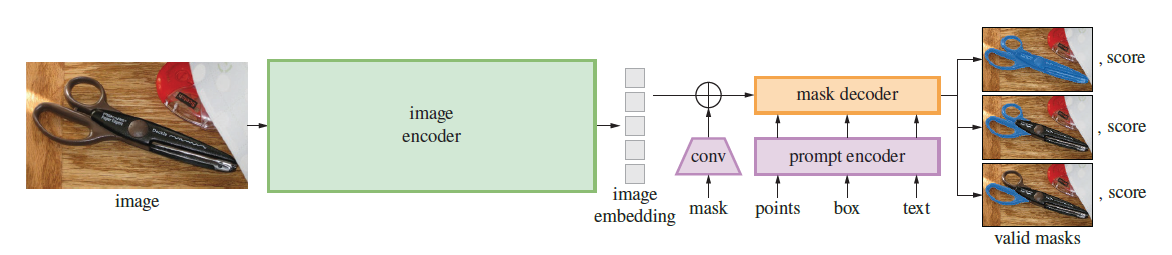
\includegraphics[width=\textwidth]{"images/sam_overview.png"}
	\caption[\texttt{SAM} Overview]{High-level overview of the two encoder networks interact to predict segmentation masks. Source: \cite{kirillov2023segment}.}
	\label{figsamoverview}
\end{figure}
A modified vision transformer \cite{dosovitskiy2020image} (ViT) is used as the image encoder. When applying ViTs the input image is divided into fixed-size patches. Each patch is embedded and treated as a token analogous to words in text tying in with the similarities to NLP. One dimensional positional encodings are added in order to retain spatial information. The image embeddings, along with positional encodings, are fed into a transformer encoder \cite{vaswani2017attention} consisting of attention blocks and feedforward neural networks, enabling the model to capture global dependencies between patches. Following the transformer encoder, the output is pooled to generate a fixed-size representation of the entire image, which is subsequently processed by fully connected layers for the final task. This approach offers benefits such as global context understanding, scalability to larger image sizes, and fewer inductive biases compared to traditional convolutional neural networks. Images are rescaled and padded to have a resoultuion of 1024x1024. The resulting image embedding output of the original vision transformer is of size 1280 x 64 x 64 and convolved twice to get to a size 256 x 64 x 64. 

While the image encoder is allowed to be computationally expensive since it only needs to be applied one time per image, both prompt encoder and mask decoder should be lightweight and fast to guarantee the ability to set many prompts and decode multiple masks at once. \texttt{SAM} allows for two types of prompts: sparse (text, boxes, points) and dense (masks) ones. As only point prompts were used in this work, only those will be discussed in the following and will simply be referred to as prompts. In order to encode the prompts, two pieces of information are required: foreground/background knowledge and positional knowledge. The positional encoding is either summed with an embedding for the foreground or one for background to form a 256 dimensional vectorial embedding.

Both types of embedding are then included into the decoder network. The decoder is depicted in Fig.~\ref{figdecoder} and its primary part consists of four steps. These four steps are performed twice to update both image and prompt embeddings. In addition to the prompt embeddings, an output token is introduced and their combinatation is then referred to as tokens. This is the only stage where there is any sort of information exchange between prompt and image. In the first step, self-attention is applied on the tokens. Afterwards the tokens are used as queries to compute the cross-attention to the image embeddings\footnote{Note that image embeddings go hand in hand with their positional embedings, too.}. As a third step, a multi-layer-perceptron (MLP) updates the tokens. Eventually, the complement of the second step is performed: the cross attention from image to tokens. The learned image embeddings, which are now aware of the prompt information, are upsampled through transposed convolutions and, at the same time, are attended to once more by the tokens. A 3-layer MLP is used to transform these tokens to a dimension so as to match the upscaled image embeddings. A pointwise product between this MLP's output and the upscaled image embeddings results in the prediction of the mask. The aforementioned output token is used within a second head to predict values for the intersection over union (IoU) to the ground truth. In order to remove ambiguity due to a given prompt, several (three by default) masks are predicted and ranked by their IoU scores. During training only masks with the highest IoU are used for the calculation of the loss.\footnote{As we only predict one mask per prompt, sorting by IoU was of little importance in this work.} 

It remains to discuss the training loop. Interactive segmentation is simulated during training by uniformly sampling a foreground point from the ground truth mask $G = (g_{i})$ and selecting subsequent points from the error region (both false positive and false negative) between the previous (binary) mask prediction $M$ and the ground truth, with each new point classified as foreground or background based on what type of error region $E$ it was sampled from. A mask prediction is provided from the previous iteration as an additional prompt, using unthresholded mask logits $P = (p_{i})$ to maximize information transfer. When multiple masks are returned, the one with the highest predicted IoU is used for the next iteration. After eight iteratively sampled points diminished returns are observed. Two additional iterations are included without new external information to allow the model to refine its predictions. One such iteration is performed at the very end and one is introduced after one randomly chosen iteration. The corresponding pseudocode can be found in App.~\ref{pcsam}. This results in a total of 11 iterations, balancing the use of external guidance with the model's own learning. This lightweight mask decoder allows for a relatively large number of iterations with minimal computational overhead compared to previous methods. The loss that is used is made up of three components: dice loss, focal loss \cite{liu2009otsu}, and IoU loss. The latter is just the penalization of the IoU prediction and is nothing but the mean squared error. The dice loss penalizes predictions by the percentage of misclassified pixels. The focal loss is a modification of the cross entropy loss with a modulation factor $\gamma$ to scale down the loss assigned to well-classified examples. All in all, the loss takes the form
\begin{equation}\label{samloss}
	L_{\text{train}} = L_{\text{dice}} + 20L_{\text{focal}}+ L_{\text{IoU}} = \left(1 - \dfrac{2|M \cap G|}{|M| + |G|}\right) - 20\sum_{i}(1-p^t_i)^{\gamma}\log p^t_i + \|\text{IoU}_{\text{pred}} - \text{IoU}_{\text{gt}}\|_{L^2}^{2},
\end{equation}
where $|\cdot|$ denotes the number of pixels of an area and the logits are defined as
\begin{equation*}
	p_i^\text{t}=\begin{cases}p&\text{if}\quad g_i=1\\1-p&\text{if}\quad g_{i}=0\end{cases},
\end{equation*}
and the summation runs over all pixels. $\gamma = 2$ was used during training.

\begin{figure}
	\centering
	\begin{subfigure}{0.45\textwidth}
		\centering
		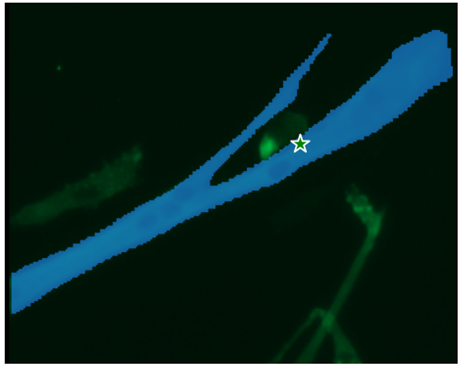
\includegraphics[width=\linewidth]{images/training1}
		\caption{First sampled foreground point from the ground truth mask}
		\label{figtrain1}
	\end{subfigure}
	\hfill
	\begin{subfigure}{0.45\textwidth}
		\centering
		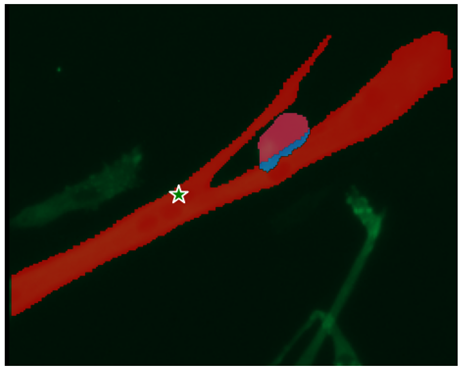
\includegraphics[width=\linewidth]{images/training2}
		\caption{Error region after the first prediction including new sampled (here: foreground) point}
		\label{figtrain2}
	\end{subfigure}
	
	\medskip
	
	\begin{subfigure}{0.45\textwidth}
		\centering
		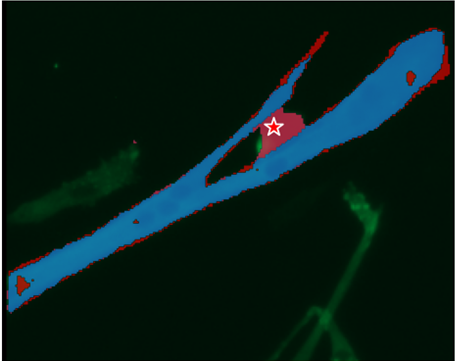
\includegraphics[width=\linewidth]{images/training3}
		\caption{New error region with another new (here: background) point prompt}
		\label{figtrain3}
	\end{subfigure}
	\hfill
	\begin{subfigure}{0.45\textwidth}
		\centering
		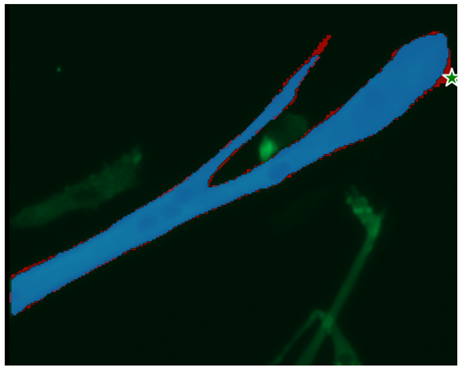
\includegraphics[width=\linewidth]{images/training4}
		\caption{Iteration beyond which resampling displays deminishing return}
		\label{figtrain4}
	\end{subfigure}
	\caption[\texttt{SAM} trainings loop]{Exemplifying the main idea behind the \texttt{SAM} training loop}
	\label{figtrain}
\end{figure}

\begin{figure}
	\centering
	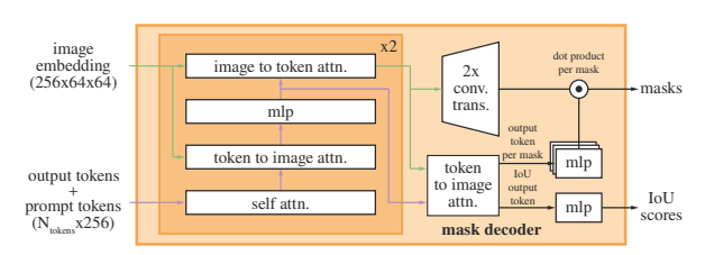
\includegraphics[width=\textwidth]{"images/maskdecoder.png"}
	\caption[\texttt{SAM} mask decoder]{Four attention steps in the mask decoder. Source: \cite{kirillov2023segment}.}
	\label{figdecoder}
\end{figure}

In order to provide a fully automated instance segmentation method without setting several prompts manually, the \texttt{SAM}AutomaticMaskGenerator class was created by Meta AI and introduced in the original publication \cite{kirillov2023segment}. This allows an instance of the class to automatically set the number of points per side, the number of crops performed before setting these points, NMS thresholds, and many other scores in order to get many masks at once.
	\newpage
	\section{Implementation and Dataset}\label{secdataset}

We developed our segmentation tool by integrating both \texttt{Stardist} and \texttt{SAM}, using \texttt{Stardist} for nuclei segmentation and a customized version of \texttt{SAM}, which we refer to as \texttt{MyoSAM}, for myotube segmentation. The primary modification in our approach involved training \texttt{MyoSAM} to enhance its capability for precise myotube segmentation. Below, we detail how each model was implemented to meet our project objectives.

\subsection{\texttt{Stardist}}
\texttt{Stardist} exceeded our expectations for nuclei segmentation, eliminating the need for additional training. We employed the ``2D\_versatile\_fluo'' model in its default configuration, which had been trained on a total of 1697 images sourced from three datasets. Two of these datasets are synthetic, designed to simulate extreme scenarios that pose significant challenges in the segmentation of cell nuclei.

\subsection{\texttt{MyoSAM} vs. \texttt{SAM}}
One distinction between \texttt{SAM} and our curated version, \texttt{MyoSAM} (short for Myovision Segment Anything Model), stems from our analysis of myotube images and their unique pixel activation patterns. Unlike \texttt{SAM}, which was designed for everyday images with different pixel distributions, \texttt{MyoSAM} required specific normalisation for the RGB channels, using mean values of red 13.21, green 21.91, blue 15.04, and standard deviations of 7.26, 16.40, and 12.12. These values differ from the ones contained in the exploratory analysis in Sec.~\ref{secexploratory} because they were calculated on both plain and preprocessed images. Additionally, given that myotubes do not possess hierarchical structures of interest, we simplified \texttt{MyoSAM} to use a single prediction head instead of three. We also limited the model to two types of prompts: point prompts to later make use of AutoMaskGenerator algorithm introduced in the original paper and discussed in Sec.~\ref{SAMbg} and mask prompts which were used to steamline the focus and improving efficiency of training.
A retained feature from \texttt{SAM} is the use of bilinear interpolation to resize input images to a standard size of 1024x1024 for compatibility with the vision transformer. For large images, \texttt{MyoSAM} employs a patching strategy similar to that described in our data labeling process. Each image is divided into patches if necessary, with \texttt{MyoSAM} predicting masks for each patch using the \texttt{SAM} Automask Generator. After segmentation, the patches are reassembled and masks are merged at split points. Finally, we calculate all relevant metrics for the segmented images, providing comprehensive data for medical analysis.


\subsection{Data Labeling}

Our project's goal is to provide medical experts specializing in the musculoskeletal domain with a tool to expedite the segmentation of myotubes, a process traditionally known for its complexity. Initially, we faced a paradox: to train a model for myotube segmentation, we required labeled data, yet obtaining this data necessitated undergoing the very labor-intensive process we aimed to streamline. At the outset, we had no labeled data at our disposal. However, inspired by the promising zero-shot performance of \texttt{SAM}, particularly its ability to recognize myotubes and their shapes, we decided to leverage it to accelerate our data annotation process, despite its tendency to produce extraneous masks. To cautiously generate labeled data suitable for training, our workflow involved several steps:

We developed a tool, that employed great zero-shot generalisation performance of \texttt{SAM}, that enabled our experts to review all predicted masks and discard any inaccuracies. This approach significantly reduced the time required for data labeling, especially when compared to manual annotation. The myotube images we worked with varied in size, from 4000x4000 pixels to as large as 9000x9000 pixels. Predicting masks on images larger than 2000x2000 pixels demanded substantial computing resources not at our disposal, causing us to adopt an image patching technique for larger images.
Given that \texttt{SAM} was trained on natural images, which differ significantly from the dark, detail-sparse backgrounds of most microscopy images, we allowed our expert to preprocess the images to improve mask prediction accuracy. Our preprocessing efforts revealed that, contrary to our initial belief, myotube microscopy images do not have a purely black background but instead ones with subtle coloring, from the markers used to visualise myotubes and nuclei. By focusing on eliminating large clusters of pixels with identical lightness based on the HSL space, we aimed to isolate the myotubes against a black background, enhancing their visibility. This preprocessing step, along with the expert validation of zero-shot generated masks, markedly accelerated the annotation process.
However, image patches needed to be reassembled into their original dimensions, requiring adjustments to the binary masks to reflect the original image accurately. This reassembly process involved stitching together myotube segments that had been divided across patches. We merged masks at horizontal and vertical divisions, dropping any masks without corresponding segments in adjacent patches and merging those with a significant overlap as measured by the intersection over union at the edges.
\texttt{SAM}'s design to accommodate prompt ambiguity led to the generation of redundant masks for the same myotube. To address this, we retained only one mask permyotube, discarding any that were completely enclosed by larger ones. Additionally, \texttt{SAM} sometimes produced disconnected masks for a single instance, which were also removed.
The refined predictions were then presented to our expert for final validation and manual completion of the segmentation process. This iterative approach to data annotation was indispensable for creating a high-quality training dataset. Without it, we would have faced significant delays in acquiring manually annotated images diverse enough to train our model effectively. This diversity is crucial to accurately represent the true data distribution of myotube microscopy images in terms of their size, color, shape, and distribution.

\subsection{\texttt{MyoSAM} Training Approach}
In developing \texttt{MyoSAM}, our training methodology was based on the original \texttt{SAM} training process, with adjustments made to accommodate the challenges of data scarcity and computational resources. This section outlines the key differences and strategies we implemented.
Our dataset comprised 19 annotated myotube images, which we divided into patches of 1500x1500 pixels. This division resulted in a total of 283 patches. To augment our dataset and increase its diversity, we applied 16 different augmentation techniques to these patches. Specifically, we performed colour jittering five times on each patch to make the training set independent of color. In terms of spatial transformations, we applied five random rotations with rotation angles between $\pm 45^{\circ}$, inverted the image, and applied both vertical and horizontal flips. This created a more isotropic dataset. In order to imitate visual distortions, we added Gaussian noise twice, and applied a Gaussian blur. These augmentation processes expanded our dataset to 4528 patches. The primary issue with the data available to us was that nearly half of the patches originated from just three images. This was due to the significant size discrepancy between these images and the other 16, leading to a skewed data distribution and exacerbating the challenge of achieving representative data variability, as illustrated in the figure on data distribution.

\begin{figure}
	\centering
	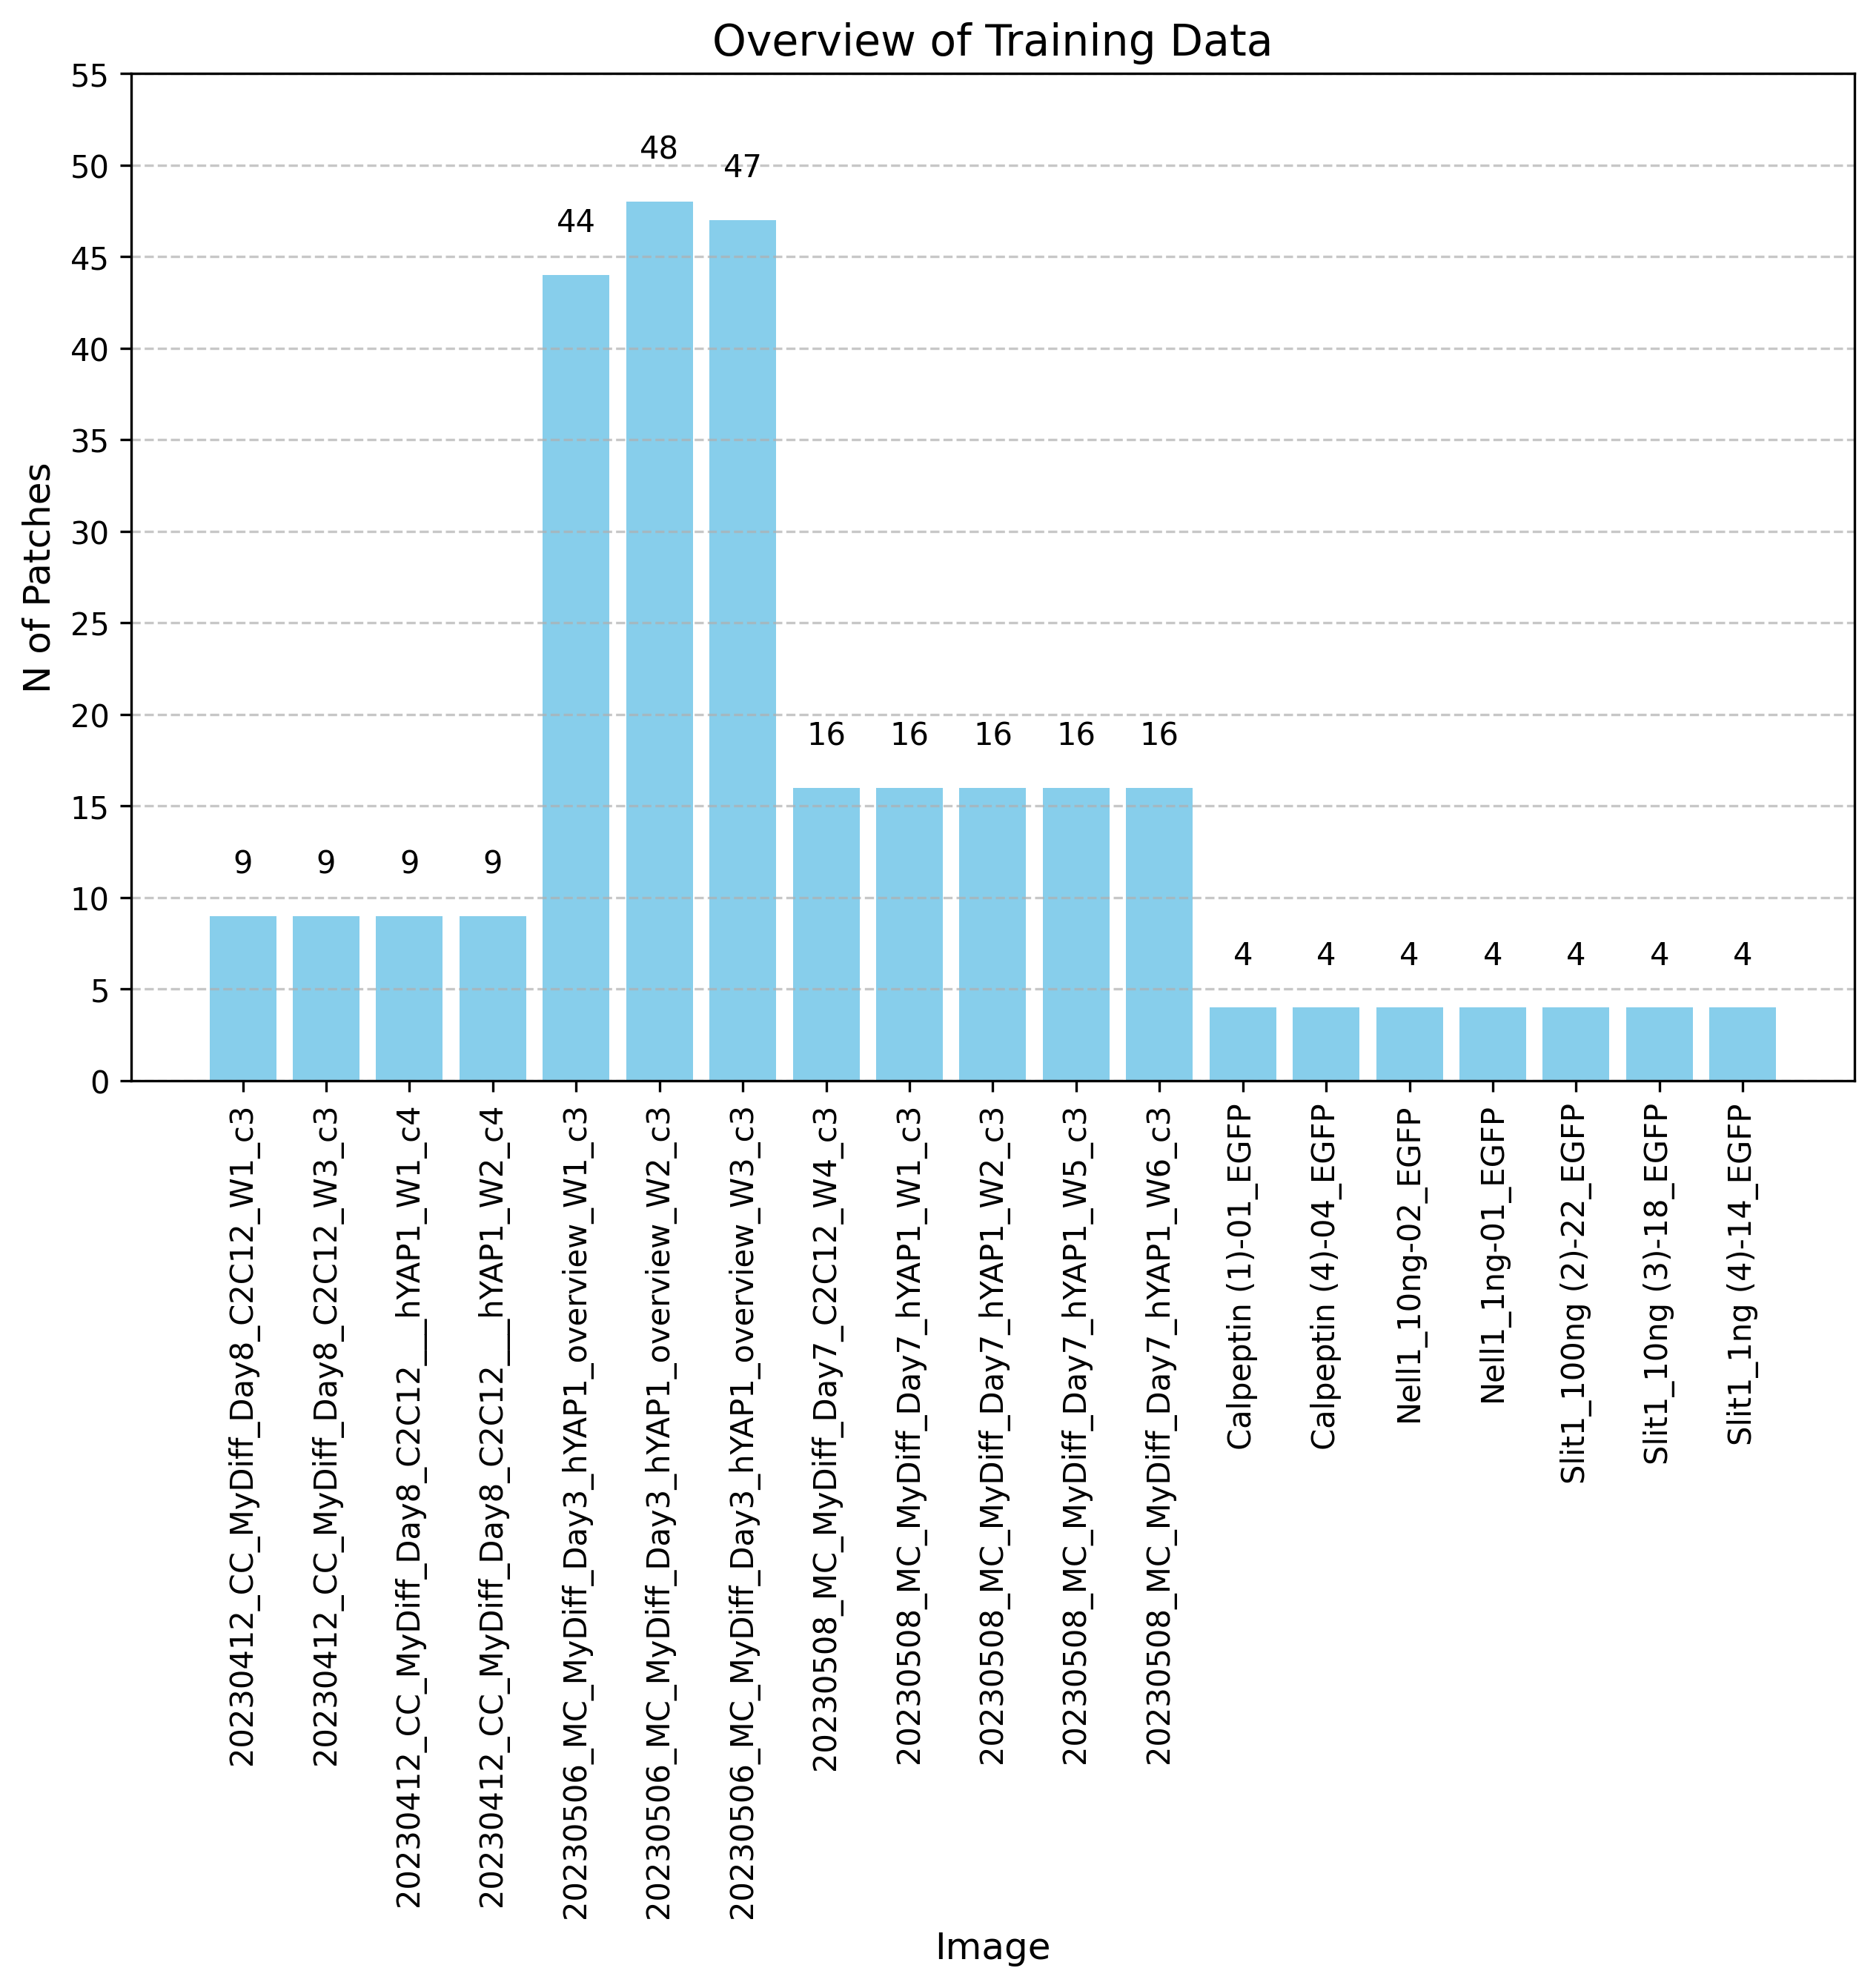
\includegraphics[width=\textwidth]{"images/overview_training_data.png"}
	\caption[TBD]{\textcolor{red}{TBD}}
	\label{figtraindata}
\end{figure}
\textcolor{red}{reffig}

We divided the augmented dataset into training (80\%) and validation (20\%) sets. To ensure a balanced distribution of images and unbiased estimation of validation error, we shuffled the patches derived from the original images before splitting to make sure that both training and validation sets contain diversified patches and all images are represented in both sets.
During training, we limited the number of instances sampled in each step to 54 in order to maintain stable memory usage and prevent out-of-memory issues. However, for validation purposes, we consistently used the same instances to ensure the comparability of validation error over time. The training was planned for 40 epochs but was terminated at the 21st epoch due to early stopping.
To enhance training efficiency and manage memory use more effectively, we utilised Automated Mixed Precision (AMP) training. Additionally, we adopted Distributed Data Parallel (DDP) training to distribute the computation across six 40GB GPUs, allowing us to parallelize the workload effectively. The training batches were configured to include six patches, corresponding to one patch per GPU, with each patch containing up to 54 instances. This setup meant that a single training step could involve processing up to 324 instances.
For optimization, we chose the AdamW optimizer with $\beta_1 = 0.9$ and $\beta_2 = 0.999$, incorporated L2 regularization with $\lambda = 0.1$ to prevent overfitting and set an initial learning rate of $10^{-4}$. We also applied a learning rate decay factor of 0.1 after every second epoch to gradually reduce the learning rate and improve convergence. The loss functions and training algorithm used in training \texttt{MyoSAM} were consistent with those used in \texttt{SAM}'s original training.


	\newpage
	\section{Performance Evaluation and Metrics}\label{secperformance}
Evaluating the performance of computer vision tasks is far from trivial. They are typically categorized into four areas: image classification, object detection, semantic segmentation, and instance segmentation, each with distinct objectives. As a result, the performance metrics applicable to one category may not be suitable for another. Moreover, each segmentation task has unique requirements and deals with different types of images, which influences the relevance of performance metrics. In our work, we focus on binary instance segmentation for both myotube and cell nuclei images. Given the distinct characteristics of these image types, we selected a set of performance metrics that we believe most accurately reflect our model's performance.
Instance segmentation tasks fundamentally involve classification, where metrics gauge a model's ability to differentiate between categories using counts of true positives, false positives, and false negatives. In binary instance segmentation, true negatives, which would correspond to the image background, are not considered. We assess our models' detection quality through metrics like precision (the rate at which predicted instances are correctly classified), recall (the ability to identify all relevant instances), and accuracy (the average of precision and recall). We also employ overlap-based metrics to compare predictions with ground truths in images and to gauge our models' segmentation quality. Metrics such as Intersection over Union (IoU), Intersection over Reference (IoR), and Normalized Surface Distance (NSD) are used, depending on the image type. These metrics are calculated for matched true positive and ground truth instances and reported both before and after normalization by the number of ground truth masks. Additionally, we report Panoptic Quality, a hybrid metric that combines segmentation and detection quality into one, yielding more conservative results due to its multiplicative factors ranging from 0 to 1. An overview over the performance metrics can be obtained in Table~\ref{tabdefs}. More detailed explanations on the quantities can be found in \cite{metricsreloaded}.


\subsection{Performance Evaluation}
In the following two subsections, we present these metrics for \texttt{Stardist}, used to segment cell nuclei, and \texttt{MyoSAM}, our model for myotube segmentation. We also juxtapose the performance of \texttt{MyoSAM} to Meta’s \texttt{SAM} model for direct comparison.
\subsubsection{Performance of Cell Nuclei Segmentation with \texttt{Stardist}}

\begin{figure}
	\centering
	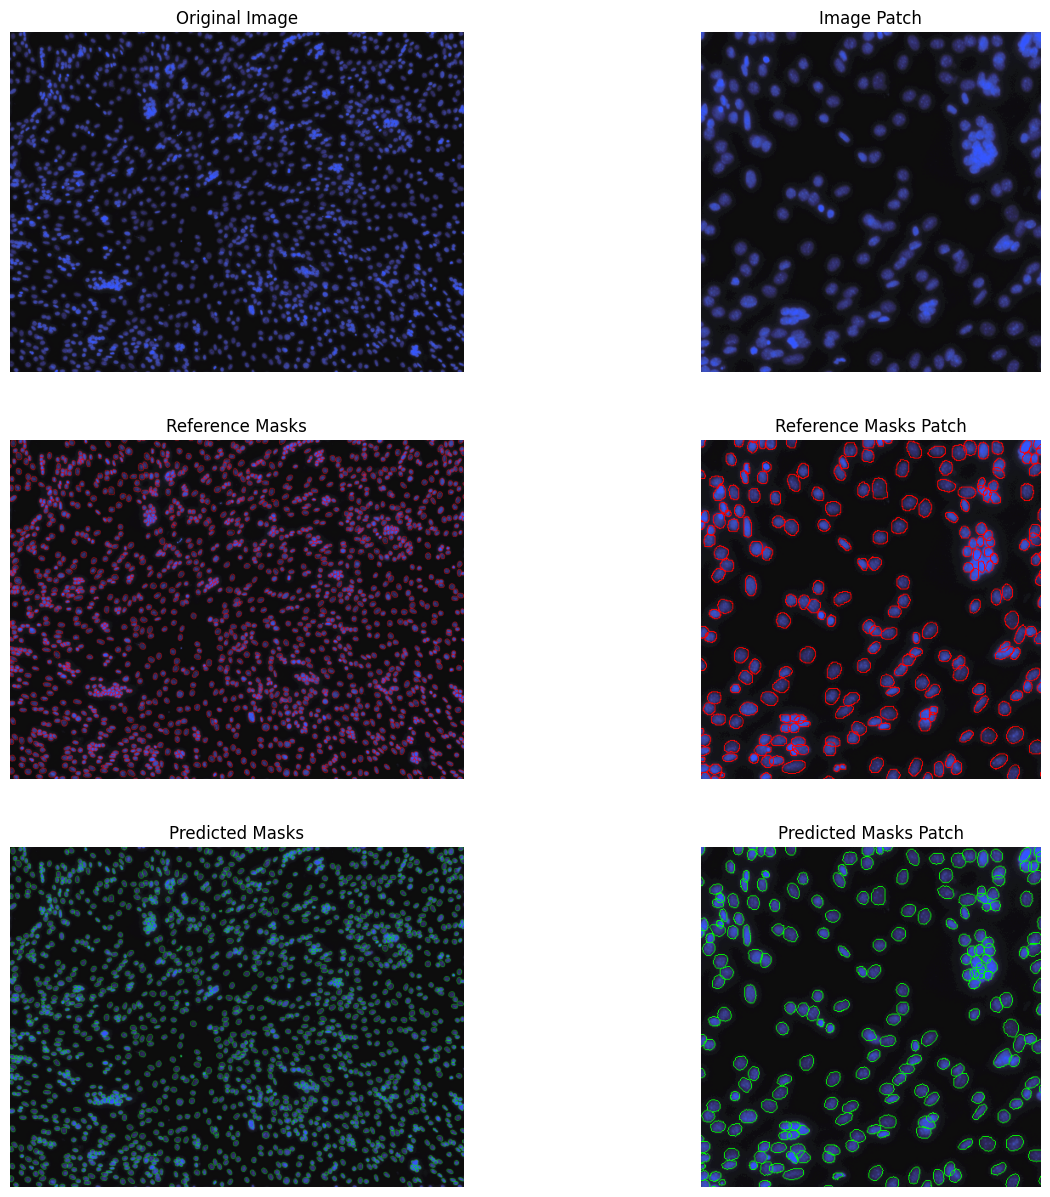
\includegraphics[width=\textwidth]{"images/qualitative_performance_stardist.png"}
	\caption[Qualitative performance \texttt{Stardist}]{Comparison of one sample image and one patch therein in terms of ground truth and \texttt{Stardist} prediction.}
	\label{figperfstardistqual}
\end{figure} 

Qualitatively, \texttt{Stardist} effectively segments cell nuclei, closely matching the shapes of manually annotated reference masks as can be seen from Fig.~\ref{figperfstardistqual}. Despite its generally precise segmentations, \texttt{Stardist} tends to slightly underestimate the number of nuclei in densely clustered areas. This observation is supported by the difference in number of reference masks ($n=1923$) compared to predicted masks ($n=1823$). To quantify this performance, we matched predictions with references using the Intersection over Reference metric, allowing less penalization for predictions that segment multiple references and accommodating single predictions to multiple references. Double assignments in matching are considered false positives.
The common threshold for mask matching in computer vision is $\tau = 0.5$, but this may be too conservative for small objects like cell nuclei, where minimal prediction shifts can noticeably impact overlap metrics. Despite this, \texttt{Stardist}'s performance remains robust even at conservative thresholds (cf. Fig.~\ref{figperfstardist} and Table~\ref{tabstardist}).


\begin{figure}
	\centering
	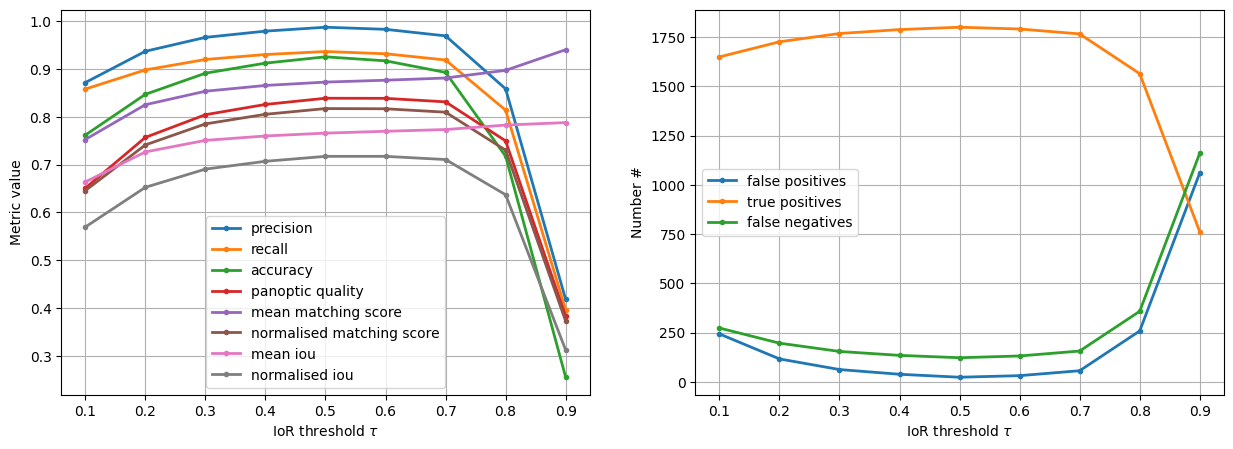
\includegraphics[width=\textwidth]{"images/quantitative_performance_stardist.png"}
	\caption[Quantitative performance \texttt{Stardist}]{Performance of \texttt{Stardist} in terms of the described metrics and ROC metrics.}
	\label{figperfstardist}
\end{figure} 

\begin{table}[H]
	\centering
	\caption{Stardist Performance ($\tau = 0.5$)}
	\label{tabstardist}
	\begin{tabular}{|l|c|}
		\hline
		True Positives & 1801 \\
		\hline
		False Positives & 23 \\
		\hline
		False Negatives & 122 \\
		\hline
		Precision & 0.99 \\
		\hline
		Recall & 0.94 \\
		\hline
		Accuracy & 0.93 \\
		\hline
		Panoptic Quality & 0.84 \\
		\hline
		Mean Matching Score (IoR) & 0.87 \\
		\hline
		Normalized Matching Score (IoR) & 0.82 \\
		\hline
		Mean IoU & 0.77 \\
		\hline
		Normalized IoU & 0.72 \\
		\hline
	\end{tabular}
\end{table}

\subsubsection{Performance of Myotube Segmentation with \texttt{MyoSAM}}

\begin{figure}
	\centering
	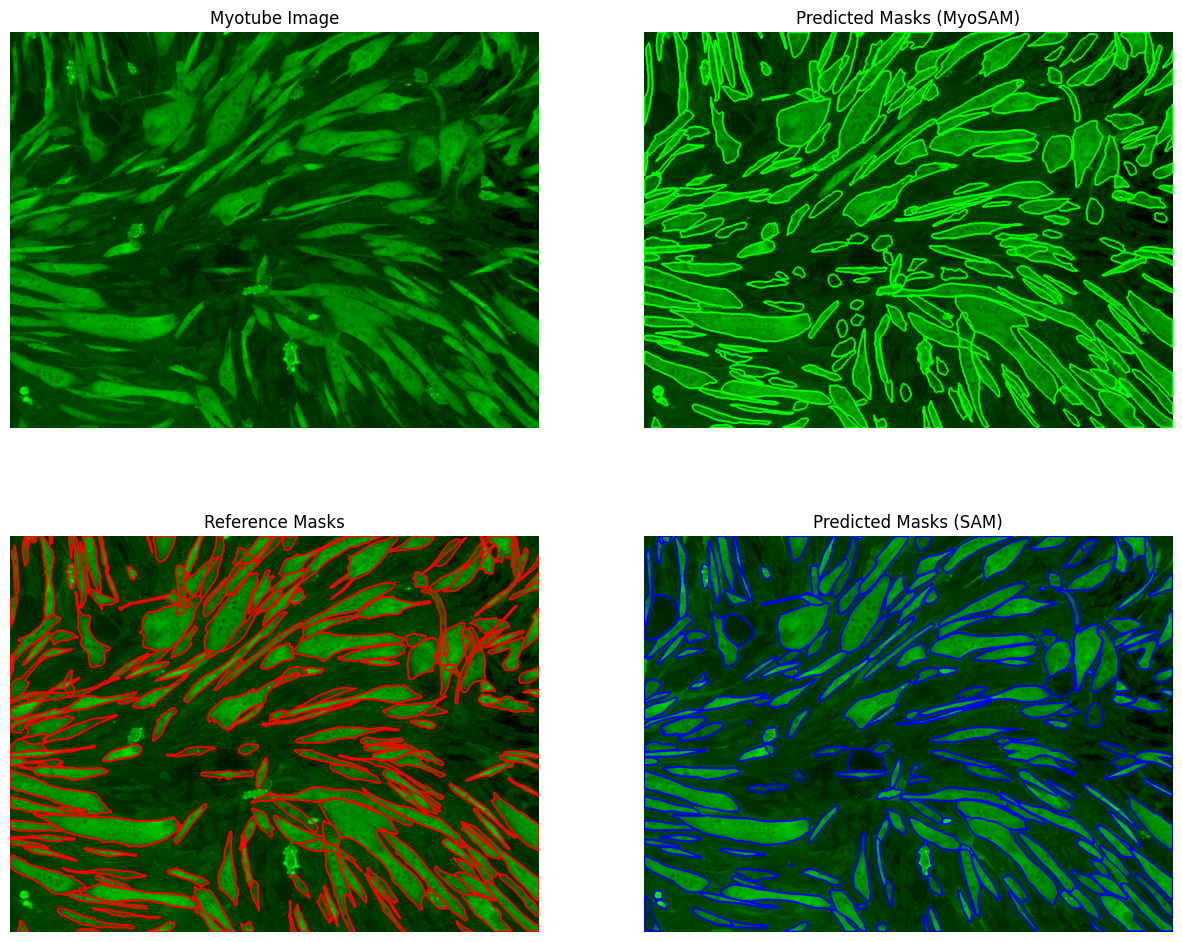
\includegraphics[width=\textwidth]{"images/qualitative_performance_myosam.png"}
	\caption[Qualitative performance \texttt{MyoSAM}]{Qualitative comparison of a myotube image with \texttt{SAM}, \texttt{MyoSAM}, and ground truth.}
	\label{figperfsamqual}
\end{figure} 
The performance comparison between \texttt{MyoSAM} and the standard \texttt{SAM} model highlights several key differences. Our focus with \texttt{MyoSAM} was on accurately delineating myotube boundaries, crucial for medical evaluations of microscopy images. To this end, we report the Normalized Surface Distance as an overlap metric for myotubes, which is a measure of overlap of the mask boundaries. NSD has an adjustable parameter $\tau_{\text{NSD}}$, with which the boundaries of both masks can be widened to account for inter-rater-variability. We set the parameter at three, meaning the boundaries were widened by three pixels both inward and outward.
Despite \texttt{SAM}'s capabilities, it faces challenges in accurately segmenting overlapping myotubes, often misidentifying them as separate entities or as disconnected parts of the same segment. Its design to segment a wide range of features results in the unnecessary segmentation of insignificant details, such as minor grains or shades within myotubes. Additionally, SAM sometimes generates redundant masks for a single myotube, a byproduct of its training to handle ambiguous prompts, despite there being no such ambiguity in myotube identification. This highlights the need for tailored approaches in myotube segmentation to avoid these specific issues. Our qualitative comparison in Fig.~\ref{figperfsamqual} shows \texttt{MyoSAM} significantly improves on these issues, but how do the metrics reflect this? We matched myotube references and predictions using IoU, and we recommend a matching threshold $\tau = 0.5$ due to the larger size of myotubes compared to nuclei. \texttt{MyoSAM} outperforms \texttt{SAM} in almost all aspects and every matching threshold except one and a slight increase in the number of predicted masks, demonstrating a quality over quantity advantage. Their individual performances are seen in Fig.~\ref{figperfsam} and Fig.~\ref{figperfsambase} while the improvement due to the training measured in terms of differences in performance metrics is seen in Fig.~\ref{figperfdiffsam}. A summary of the metrics for $\tau = 0.5$ can be found in Table~\ref{tabmyosamvssam}.
\begin{table}[H]
	\centering
	\caption{MyoSAM vs SAM ($\tau = 0.5$)}
	\label{tabmyosamvssam}
	\begin{tabular}{|l|c|c|c|}
		\hline
		Metric & MyoSAM & SAM & Difference \\
		\hline
		True Positives & 169 & 161 & 8.00 \\
		\hline
		False Positives & 65 & 69 & -4.00 \\
		\hline
		False Negatives & 43 & 51 & -8.00 \\
		\hline
		Precision & 0.72 & 0.7 & 0.02 \\
		\hline
		Recall & 0.79 & 0.76 & 0.03 \\
		\hline
		Accuracy & 0.61 & 0.57 & 0.04 \\
		\hline
		Panoptic Quality & 0.62 & 0.57 & 0.05 \\
		\hline
		Mean Matching Score & 0.81 & 0.78 & 0.03 \\
		\hline
		Normalized Matching Score & 0.65 & 0.59 & 0.06 \\
		\hline
		Mean NSD & 0.88 & 0.83 & 0.05 \\
		\hline
		Normalized NSD & 0.7 & 0.63 & 0.07 \\
		\hline
	\end{tabular}
\end{table}
\begin{figure}
	\centering
	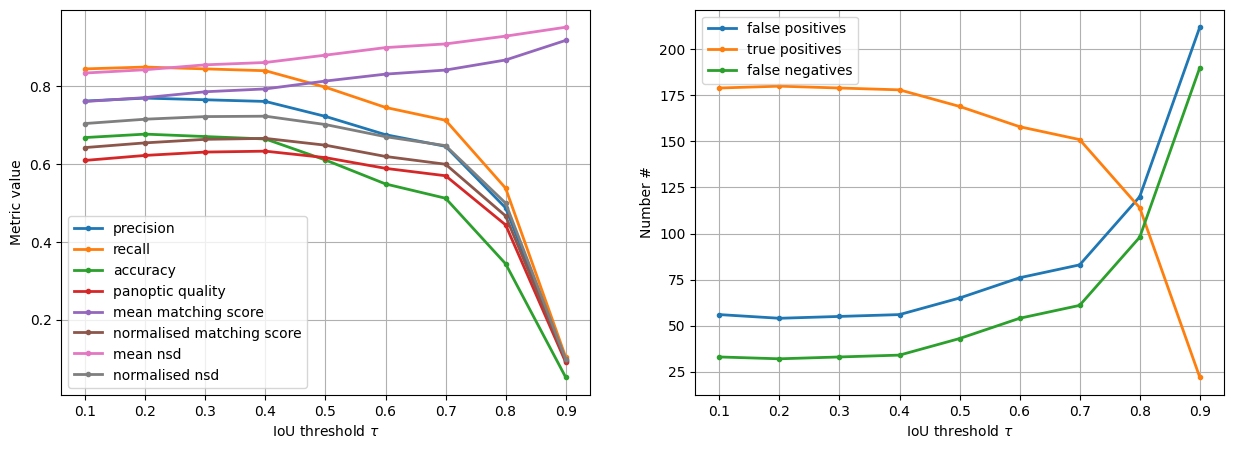
\includegraphics[width=\textwidth]{"images/quantitative_performance_myosam.png"}
	\caption[Quantitative performance \texttt{MyoSAM}]{Performance of \texttt{MyoSAM} in terms of the described metrics and ROC metrics.}
	\label{figperfsam}
\end{figure}
\begin{figure}
	\centering
	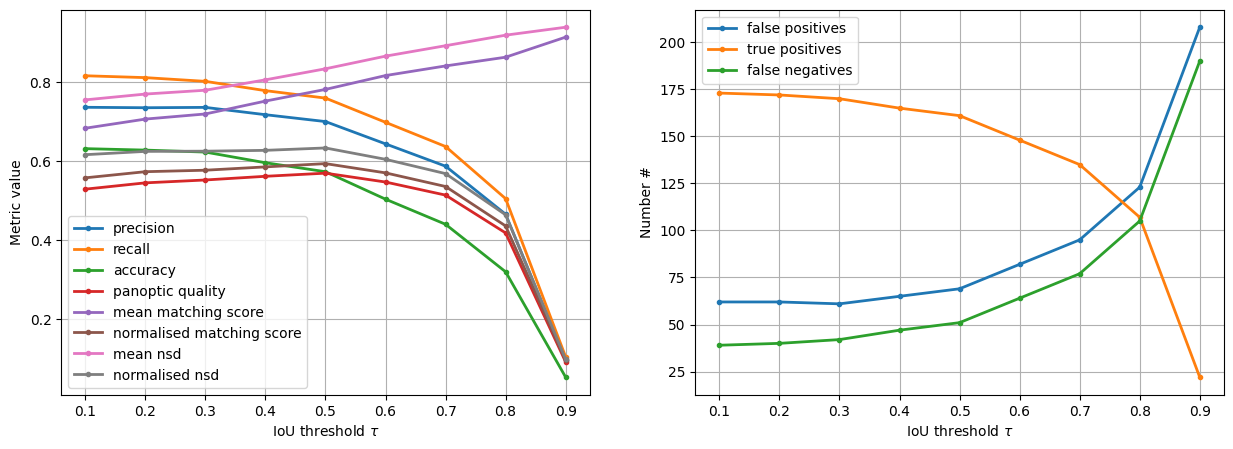
\includegraphics[width=\textwidth]{"images/quantitative_performance_sam.png"}
	\caption[Quantitative performance \texttt{SAM}]{Performance of \texttt{SAM} in terms of the described metrics and ROC metrics.}
	\label{figperfsambase}
\end{figure}
\begin{figure}
	\centering
	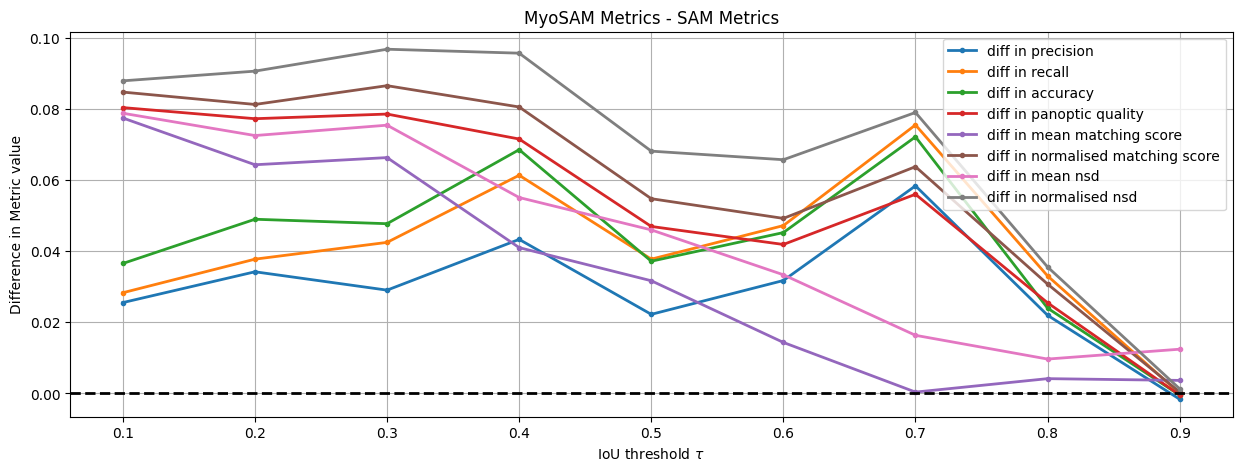
\includegraphics[width=\textwidth]{"images/diff_quantitative_performance_myosam_sam.png"}
	\caption[Difference quantitative performance \texttt{SAM} and \texttt{MyoSAM}]{Performance differences between \texttt{MyoSAM} and \texttt{SAM}.}
	\label{figperfdiffsam}
\end{figure} 


\subsection{Myovision Metrics}
Our research involves segmenting microscopic myotubes and cell nuclei, a process crucial for musculoskeletal researchers and medical practitioners. This segmentation allows for detailed analysis and understanding of myotubes and cell nuclei, providing valuable insights into muscular health and diseases. To support this analysis, our tool has been developed to offer a wide range of metrics in real-time to facilitate a speedy examination with no human error. We offer a total of 31 metrics, divided into image-specific and myotube-specific categories, as detailed in Table~\ref{tabimgspec} and Table~\ref{tabmyospec}.
\subsubsection{Image Specific Metrics}
These metrics primarily count the instances of various musculoskeletal components within an image. Myoblasts are defined as nuclei not contained within a myotube. A nucleus is considered part of a myotube if 95\% or more of its area is inside the myotube. This determination involves a multi-step process, starting with identifying if nuclei centroids are within a myotube's bounding box, then verifying if their centroids are within the myotube's perimeter. We further refine this by converting the relevant myotubes and nuclei into a binary mask to check the percentage of a nucleus's area inside a myotube. However, the masks we create correspond to the size of the myotube’s bounding box instead of the whole image thus optimizing memory usage. Clusters of nuclei within the same myotube are identified by detecting overlaps and creating a graph where nuclei are nodes connected by their overlaps using \cite{hagberg2008exploring, hagberg2020networkx}. The number of nodes in this graph represents the number of nuclei in a cluster. Area measurements for myotubes, nuclei, and myoblasts are obtained by counting the pixels within each entity, allowing for conversion to metric scale measurements if the pixel size in the microscopic image is known.
\subsubsection{Myotube Specific Metrics}
These metrics include the predicted Intersection over Union (IoU) and Stability, both built in \texttt{SAM} metrics. Predicted IoU measures the predicted overlap between predicted and reference masks, while Stability assesses the sensitivity of predicted masks to changes in prompts. Pixel activation metrics (such as RGB min, max, mean, median, mode, and standard deviation) provide color intensity information across three channels. The integrated RGB density metric sums the pixel intensities for each color channel. Shape descriptors like Area, Convex Area, Solidity, Aspect Ratio, Roundness, Perimeter, Feret’s Diameter, and Circularity offer detailed insights into each myotube's physical characteristics. For example, Convex Area is calculated from the area enclosed by the convex hull of a myotube, while Solidity and Roundness measure convexity and circularity, respectively. Feret's Diameters, both minimum and maximum, are derived from linear projections of myotubes using their eigenvectors, measuring their diameter in the directions of minimum and maximum variance. The Instance Fusion Index quantifies the number of nuclei within a specific myotube. Lastly, each myotube is accompanied by cluster information, detailing the number of clusters within a myotube and the number of nuclei in each cluster, along with their indicators.
This comprehensive suite of metrics provided by our \texttt{MyoSAM} tool is designed to facilitate a deeper understanding and analysis of myotubes and their cellular components, offering a robust framework for musculoskeletal research and medical diagnostics.



	\newpage
	\section{Conclusion and Outlook}
In our exploration of models for segmenting myotube images and their corresponding cell nuclei, Stardist emerged as highly efficient with minimal need for modification. Its success can be attributed to the relatively homogeneous shapes of nuclei, which align well with methods that rely on rigid shape approximation. On the other hand, SAM, despite living up to its reputation as a foundational model through its impressive zero-shot performance, required further training to fully automate our segmentation approach. This necessity led to the development of MyoSAM. Our objective was to create a tool, facilitating both inference and labelling tasks, accessible to medical experts without the need for programming expertise. MyoSAM was integrated into our tool in versatile ways, supporting automatic segmentation via the auto mask generator and enabling interactive segmentation. Both functionalities significantly streamline the segmentation process of myotube images. Recognizing the scarcity of labelled data in this domain, we have made our dataset and training code publicly available, hoping to spur further advancements in the field of musculoskeletal research.

However, MyoSAM, while effective, is not without its limitations. The primary challenge lies in the scarcity and lack of diversity in our dataset, which comprised only 19 annotated images. These images do not adequately represent the wide variability in myotubes, characterised by their complex and heterogeneous shapes, sizes, and colours. Additionally, our training was constrained by limited computational resources, restricting our ability to conduct extensive experiments, such as hyperparameter optimization.
We encourage domain experts to use our annotation tool to gather more data, highlighting the critical need for MyoSAM to be trained on a more diverse and expansive dataset. While we considered the entire SAM model for fine-tuning, more targeted approaches, such as adapter tuning techniques like LoRA or focusing on specific network components, may offer more efficient pathways for improvement. Optimising the auto mask generator, which underpins the automatic segmentation functionality, could enhance replicability and segmentation quality, tailored to general or specific use cases. Moreover, training lightweight architectures like U-Net, utilising our tool for data generation, presents an alternative strategy worth exploring.
Despite these challenges, we are encouraged by the advancements MyoSAM represents over SAM, especially considering the limited size of our dataset. MyoSAM mitigates human error and inter-rater variability, paving the way for more consistent and replicable analyses. This project marks a promising beginning, with ample room for improvement through training on larger, more representative datasets. We are optimistic about the potential and current capabilities of our tool.

	\newpage
	%\pagenumbering{gobble}
	\printbibliography
	\appendix
	\cleardoublepage
	\section{Appendix}
\textcolor{red}{Add references to Figures in text}

\subsection{Trainings Loop}\label{pcsam}
\begin{algorithm}
	\caption{SAM Training Algorithm}
	\begin{algorithmic}[1]
		\State Initialize ground truth mask $G$
		\State Initialize total number of iterations $n$
		\State Initialize logit mask $ P = \text{None}$
		\State Initialize threshold $t$
		\State Sample random integer $u\in \{k \in \mathbb{N}|k\leq n\}$
		\State Uniformly sample a foreground point $p$ from $G$
		\For{$i = 1$ to $n$}
		\State Predict new logit mask $P$ using point $p$ and logit mask $P$
		\If{i = u or i = n}
		\State \textbf{continue}
		\EndIf
		\State Update binarized mask $M_{\text{pred}} = P > t$ 
		\State Update error region $E = |G - M_{\text{pred}}|$
		\State Update point $p$ by sampling uniformly from error region $E$
		\If{$E(p)$ is false negative}
		\State $p$ is a foreground point
		\ElsIf{$E(p)$ is false positive}
		\State $p$ is a background point
		\EndIf
		\EndFor
	\end{algorithmic}
\end{algorithm}
\subsection{Losses and Learning Rate}\label{seclr}
\begin{figure}[H]
	\centering
	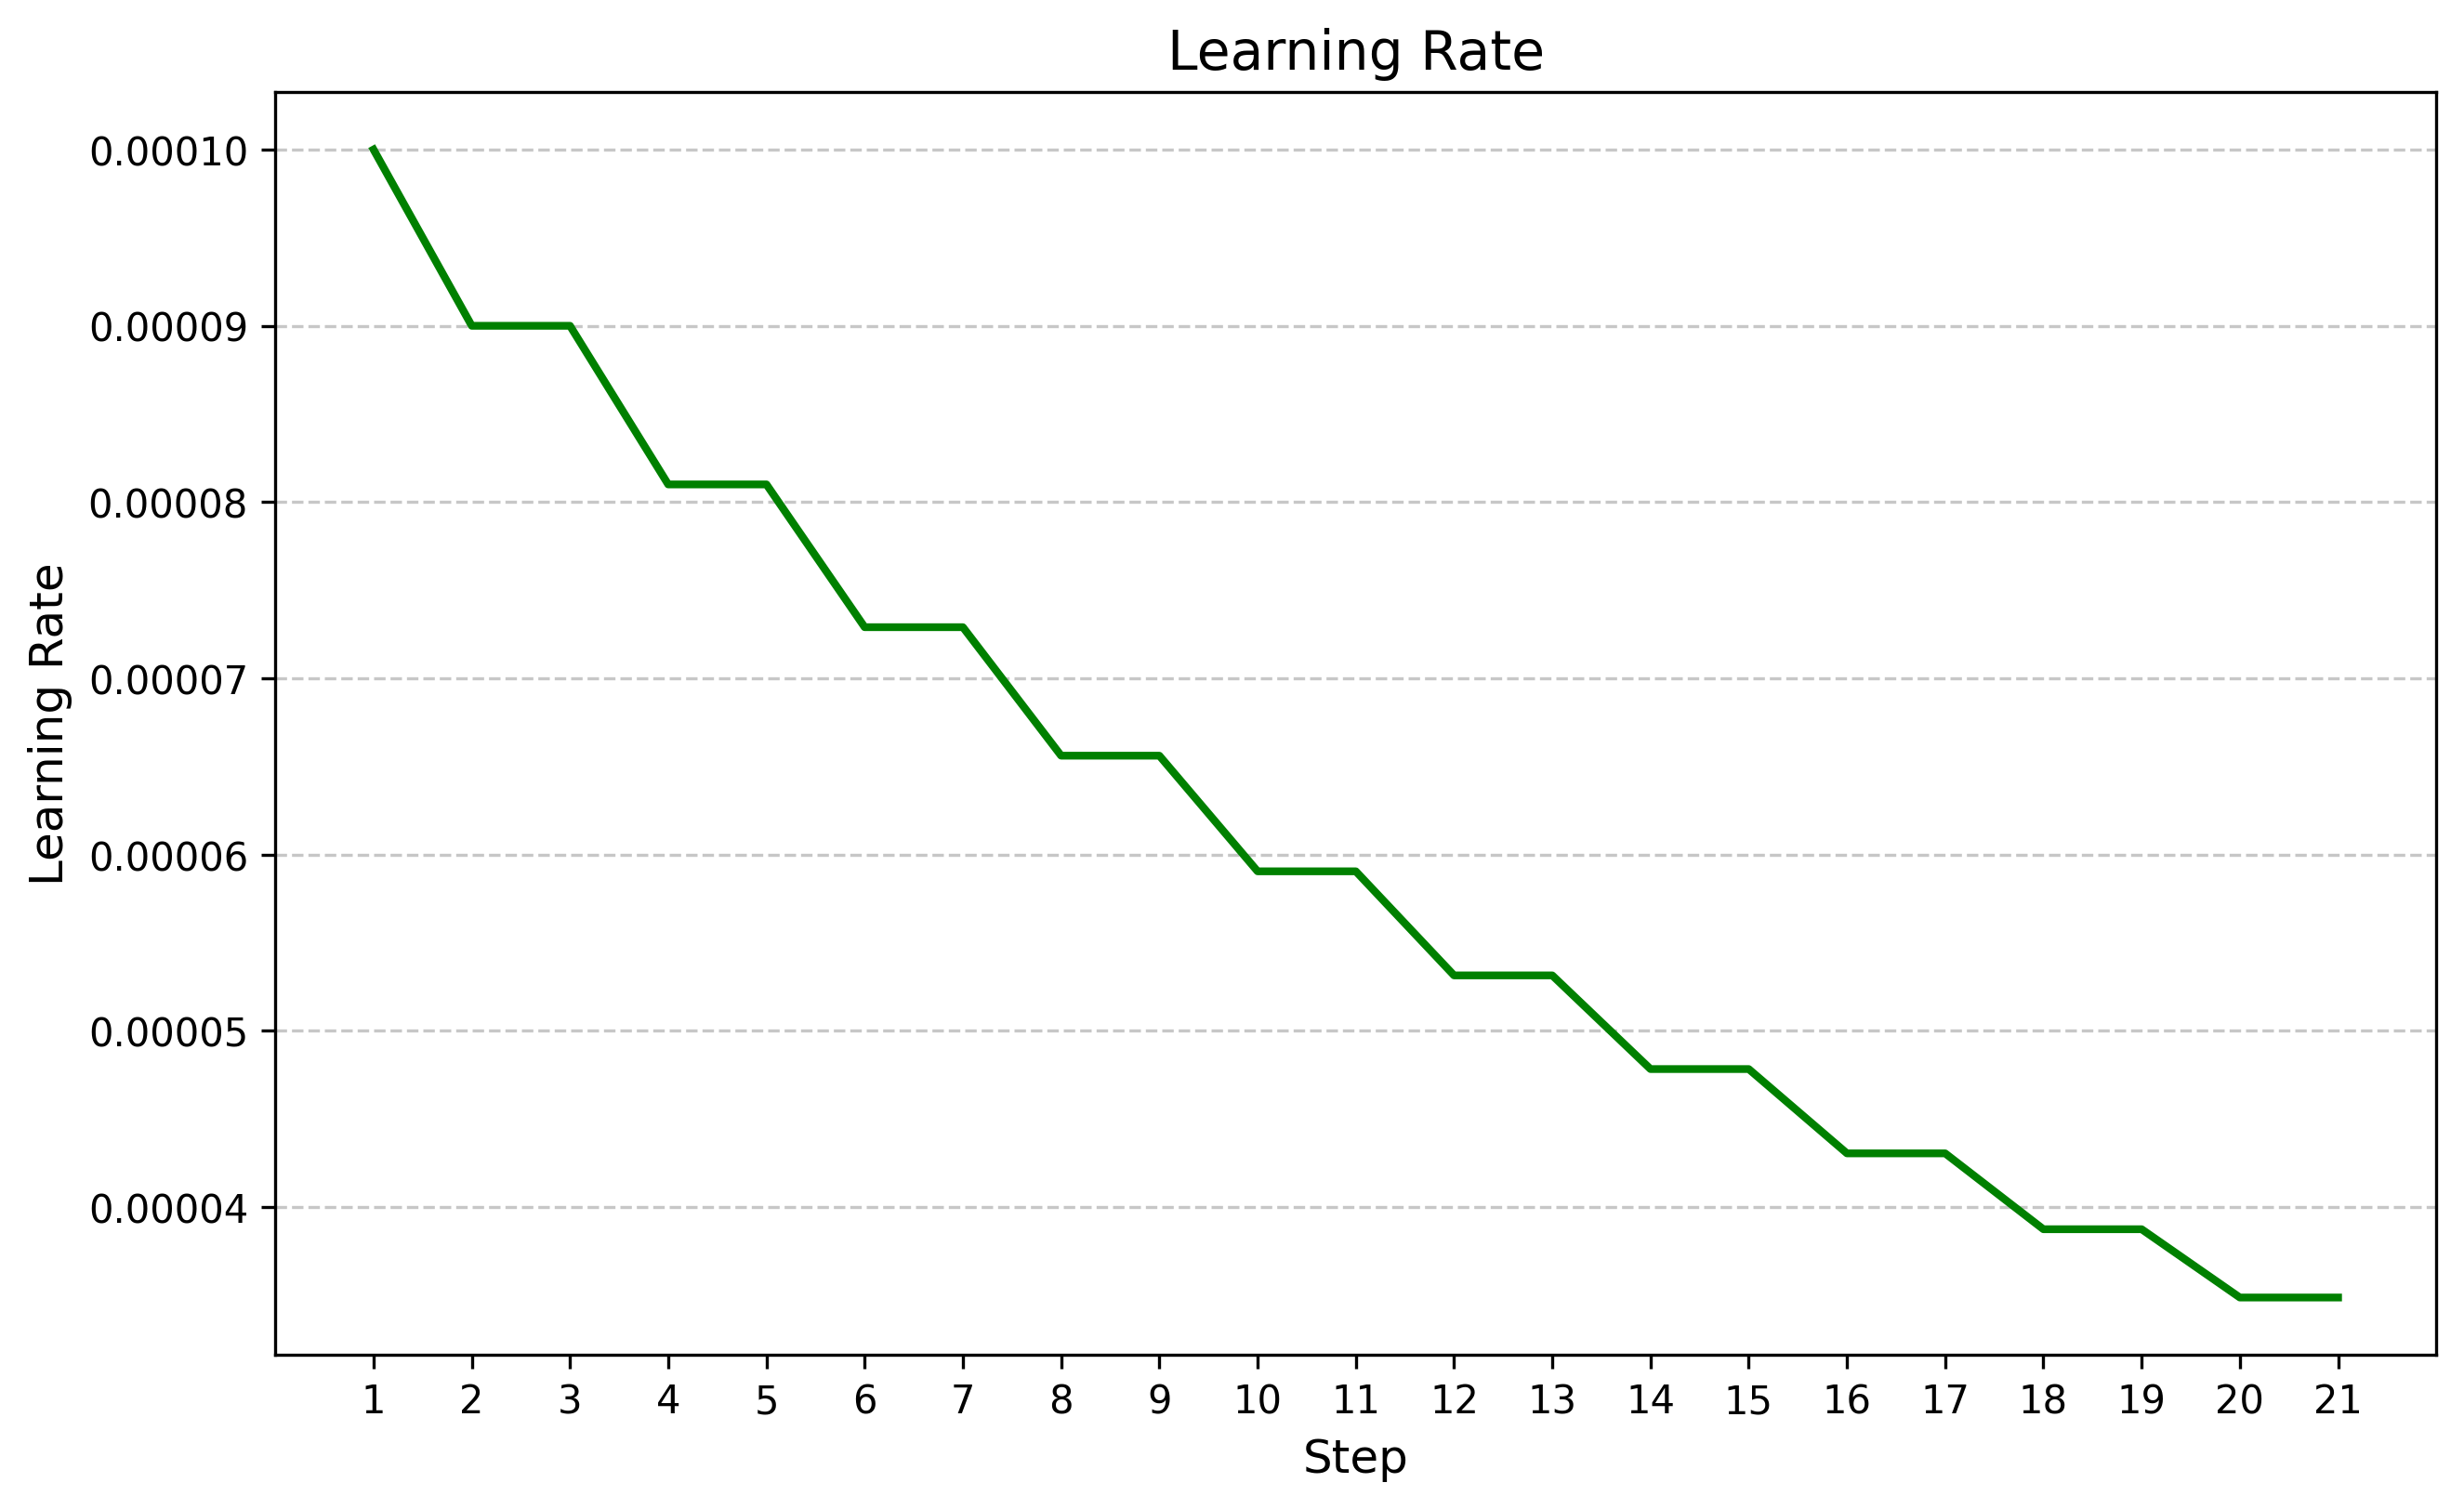
\includegraphics[width=\textwidth]{"images/lr.png"}
	\caption[Learning rate \texttt{MyoSAM}]{Progression of \texttt{MyoSAM} learning rate.}
	\label{figlr}
\end{figure}
\begin{figure}[H]
	\centering
	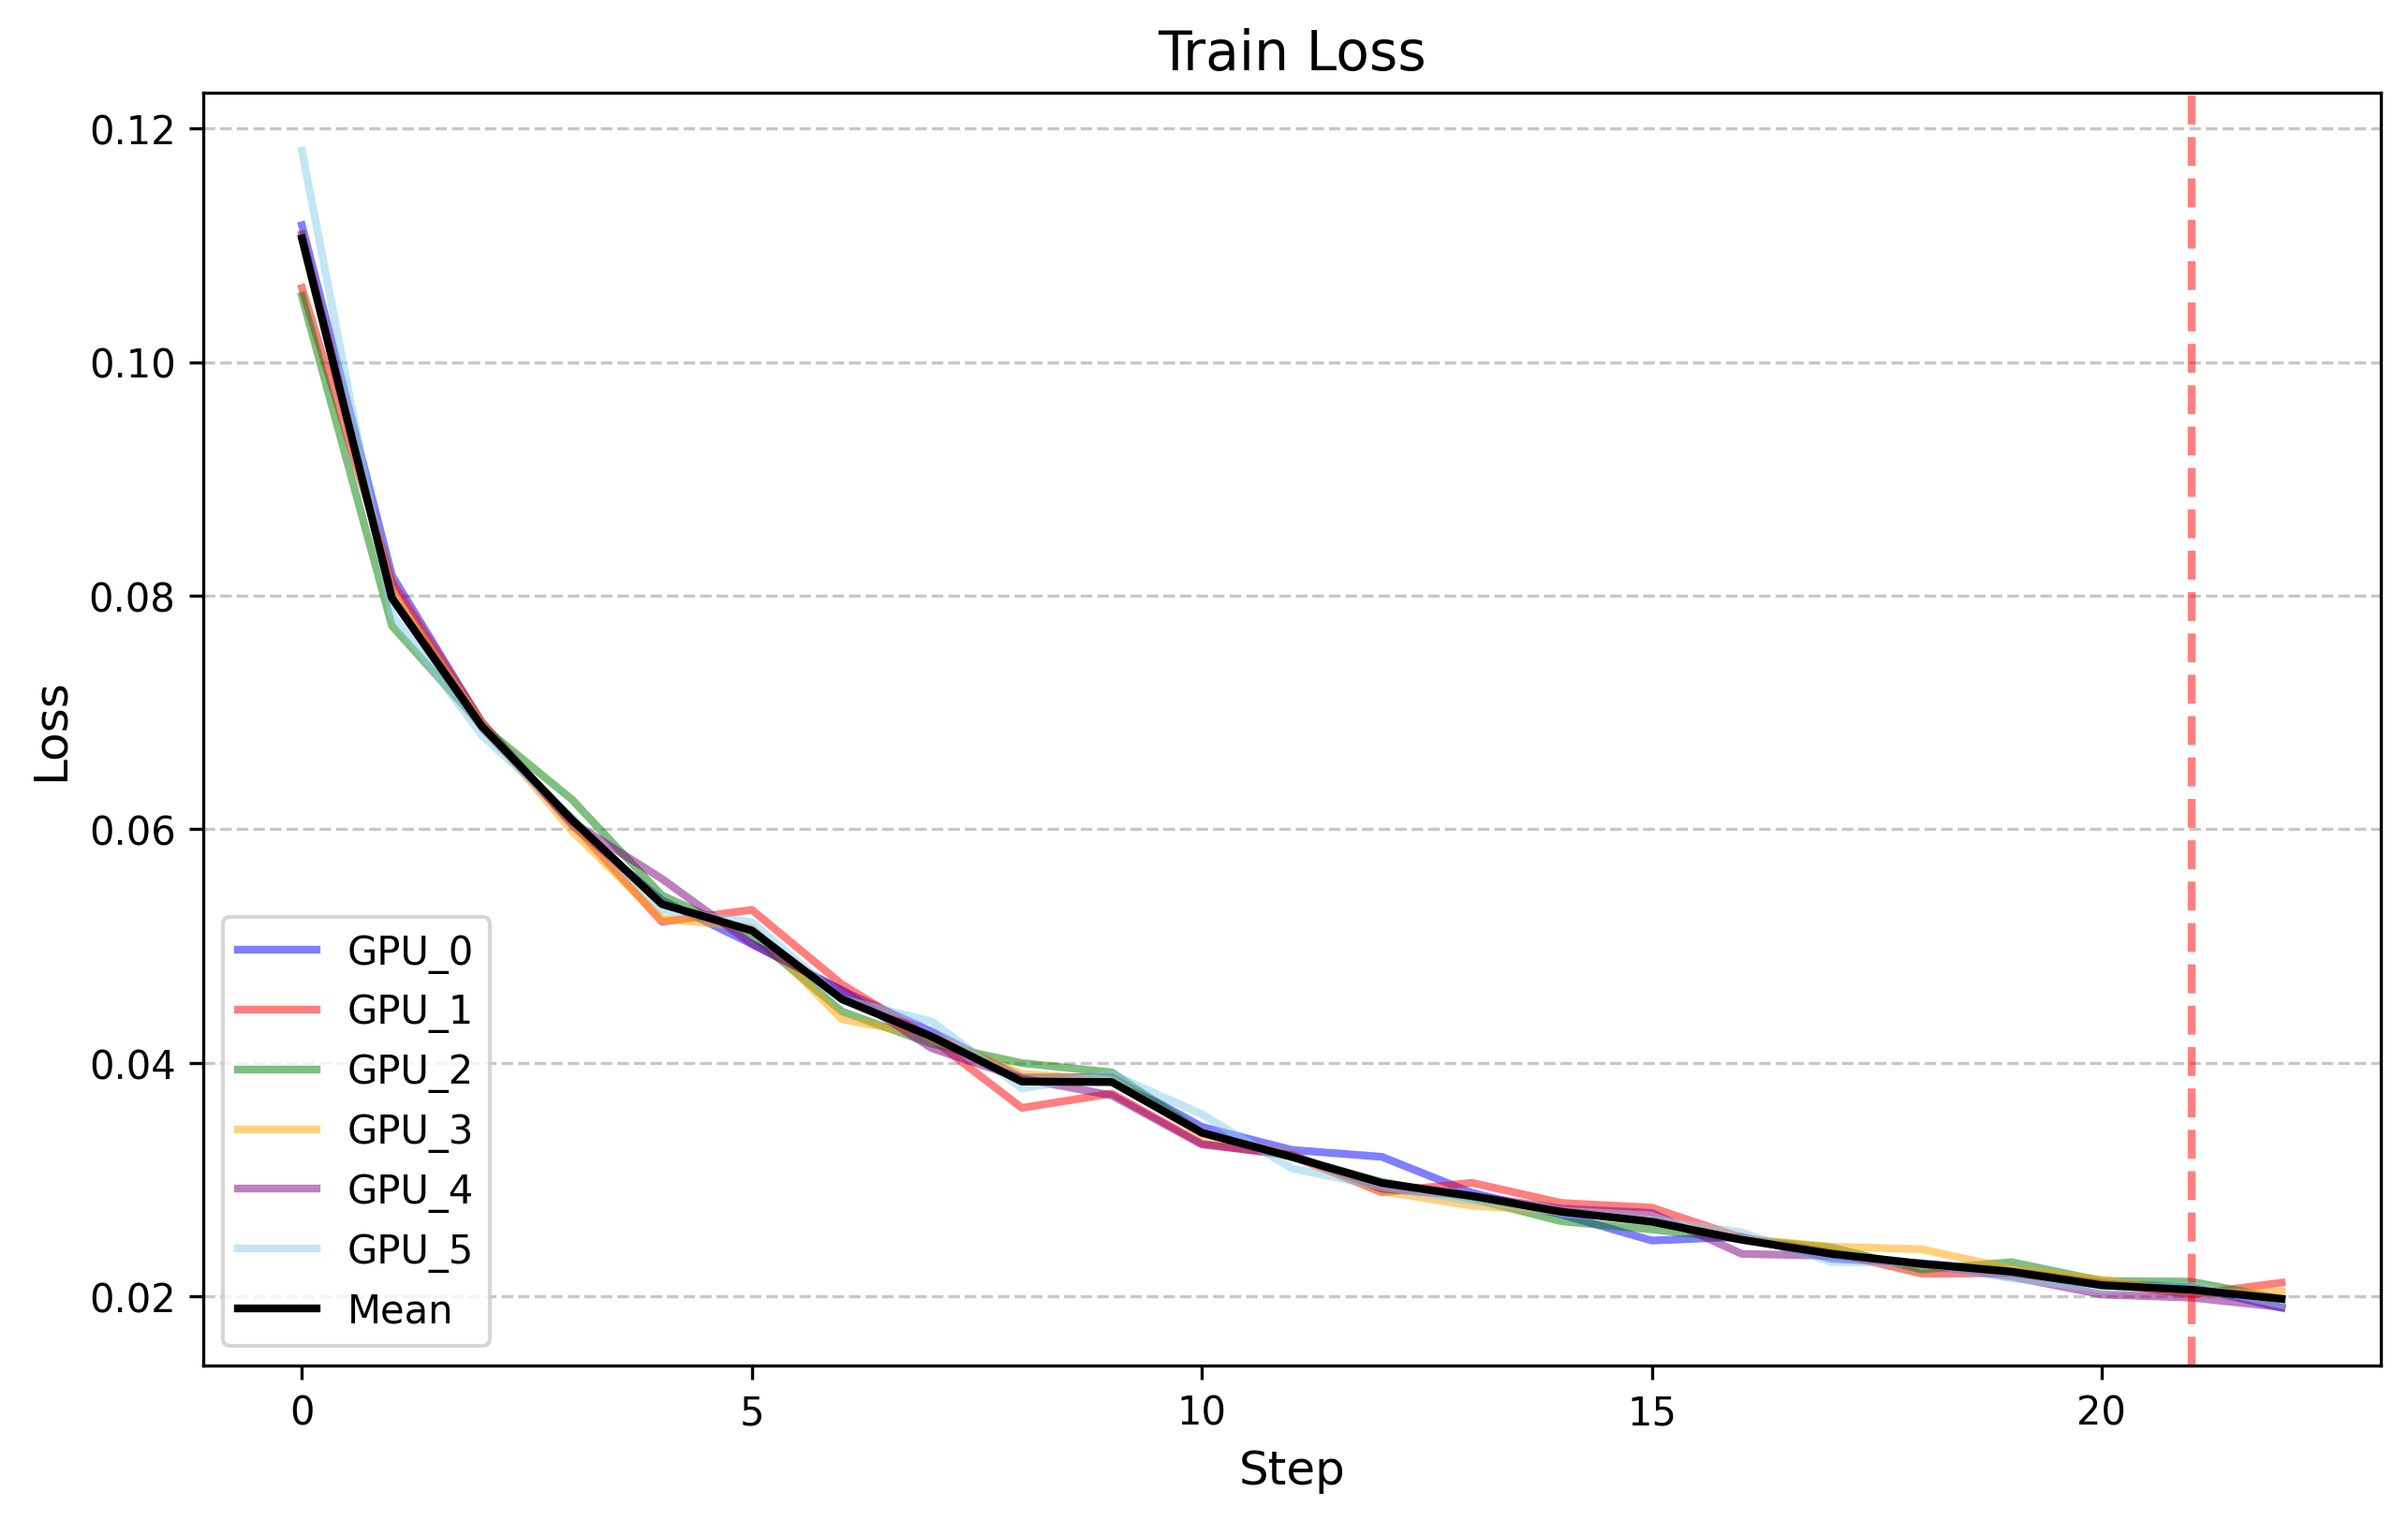
\includegraphics[width=\textwidth]{"images/train_loss.png"}
	\caption[Train loss \texttt{MyoSAM}]{Progression of \texttt{MyoSAM} train loss.}
	\label{figtrainloss}
\end{figure}
\begin{figure}[H]
	\centering
	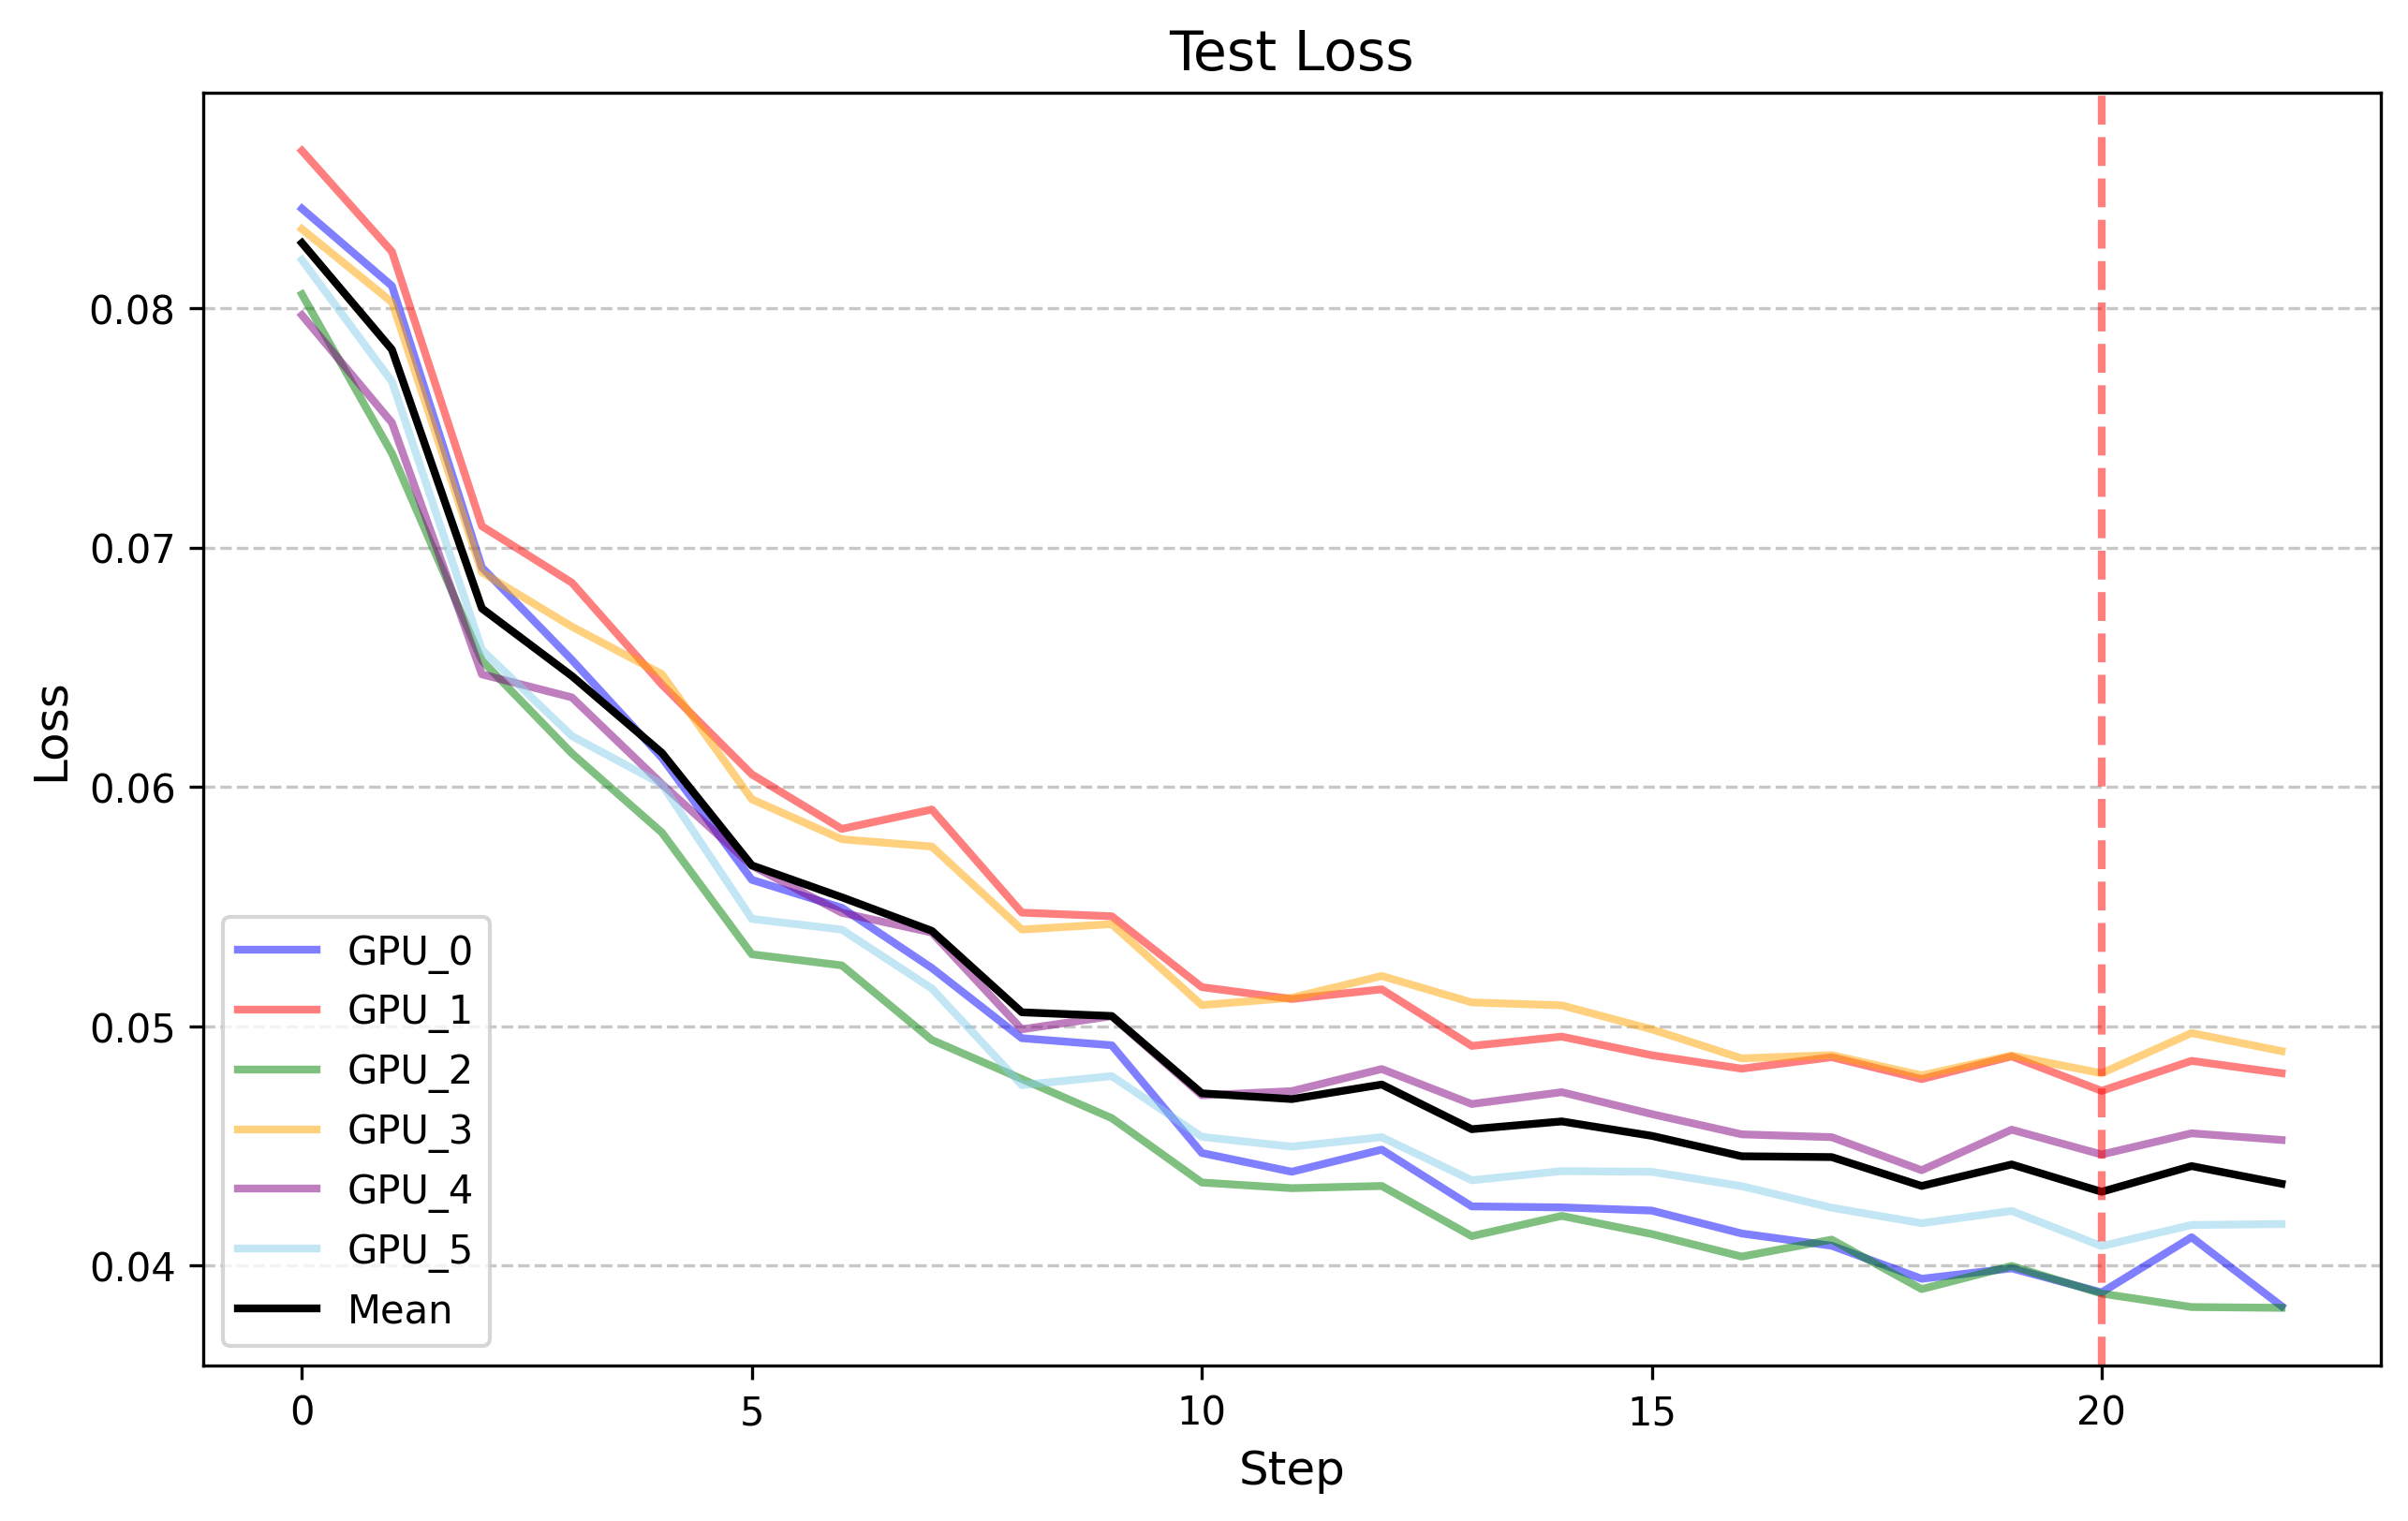
\includegraphics[width=\textwidth]{"images/test_loss.png"}
	\caption[Test loss \texttt{MyoSAM}]{Progression of \texttt{MyoSAM} test loss.}
	\label{figtestloss}
\end{figure}
\begin{figure}
	\centering
	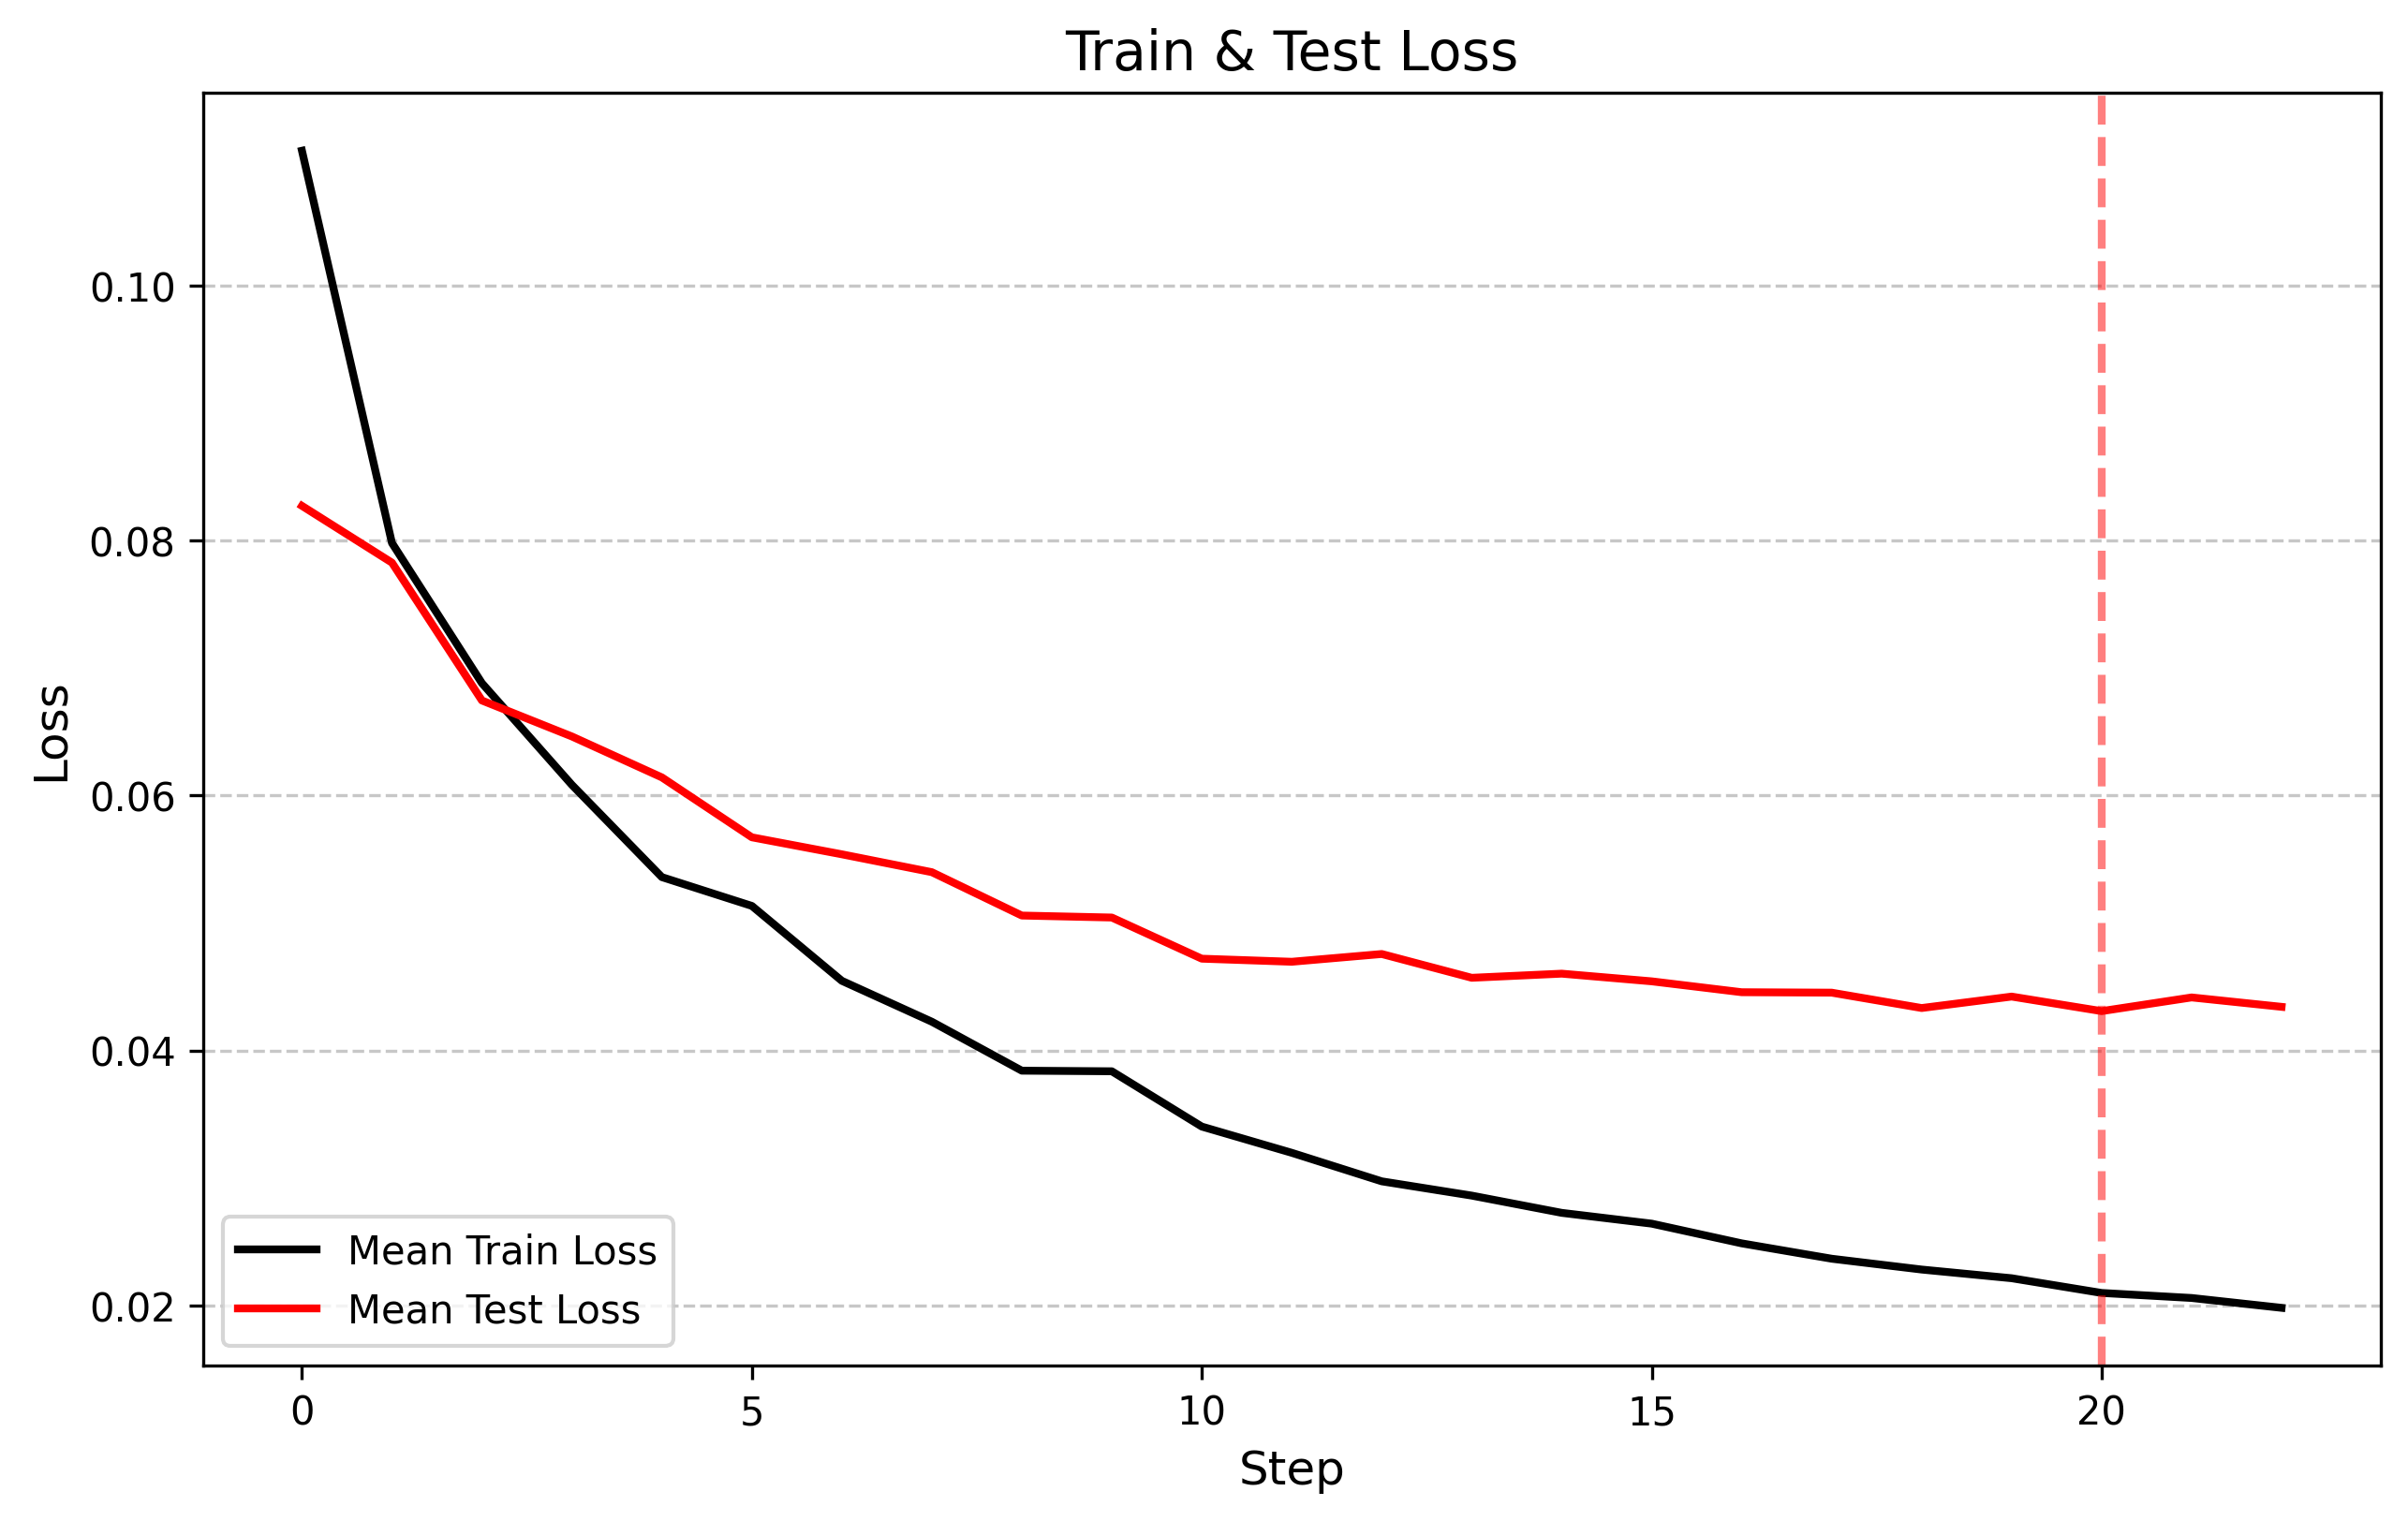
\includegraphics[width=\textwidth]{"images/train_test_loss.png"}
	\caption[Train and Test loss \texttt{MyoSAM}]{Comparison of \texttt{MyoSAM} loss progression.}
	\label{figtraintestloss}
\end{figure}
\subsection{Metrics}\label{secmetrics}
% Table 1: Image Specific Metrics
\begin{table}[H]
	\centering
	\caption{Image Specific Metrics}
	\begin{tabular}{|l|c|}
		\hline
		Metric & Formula \\
		\hline
		Total myotubes &  \\
		\hline
		Total nuclei &  \\
		\hline
		Total myoblasts &  \\
		\hline
		Total nuclei inside myotubes &  \\
		\hline
		Total fusion index & Total Fusion Index = $\frac{\text{N Nuclei in Myotubes}}{\text{N Nuclei}}$ \\
		\hline
		Number of nuclei clusters &  \\
		\hline
		Total myotube area &  \\
		\hline
		Total nuclei area &  \\
		\hline
		Total myoblasts area &  \\
		\hline
		Total nuclei inside myotubes area &  \\
		\hline
	\end{tabular}
\end{table}

% Table 2: Myotube Specific Metrics
\begin{table}[H]
	\centering
	\caption{Myotube Specific Metrics}
	\begin{tabular}{|l|c|}
		\hline
		Metric & Formula \\
		\hline
		Predicted IoU & IoU = $\frac{\text{Area of Overlap}}{\text{Area of Union}}$ \\
		\hline
		Stability &  \\
		\hline
		Is on edge &  \\
		\hline
		RGB min &  \\
		\hline
		RGB max &  \\
		\hline
		RGB mean &  \\
		\hline
		RGB median &  \\
		\hline
		RGB mode &  \\
		\hline
		RGB standard deviation &  \\
		\hline
		Integrated density RGB &  \\
		\hline
		Area &  \\
		\hline
		Convex area &  \\
		\hline
		Solidity & Solidity = $\frac{\text{Area}}{\text{Convex Area}}$ \\
		\hline
		Aspect ratio &  \\
		\hline
		Roundness & Roundness = $\frac{4 \times \text{Area}}{\pi \times \text{Major Axis}^2}$ \\
		\hline
		Perimeter &  \\
		\hline
		Feret’s Diameter (min \& max) &  \\
		\hline
		Circularity & Circularity = $\frac{4 \pi \times \text{Area}}{\text{Perimeter}^2}$ \\
		\hline
		Instance fusion index &  \\
		\hline
		Centroid &  \\
		\hline
		Cluster information &  \\
		\hline
	\end{tabular}
\end{table}
\end{document}